\documentclass[a4paper,twoside,openany]{book}
%\documentclass[aps,prl,preprint,groupedaddress]{revtex4}
%\documentclass[prl,nobibnotes,superscriptaddress,prb]{revtex4}
%%%%%%%%%%%%%%%%%%%%%%%%%%%%%%%%%%%%%%%%%%%%%%%%%%%%%%%%%%%%%%%%%%%%%%%%%%%%%%%%%%%%%%%%%%%%%%%%%%%%%%%%%%%%%%%%%%%%%%%%%%%%
\usepackage{amsmath}
\usepackage{amssymb,graphicx}
%\usepackage{apstemplate}
%TCIDATA{OutputFilter=LATEX.DLL}F
%TCIDATA{Created=Fri Aug 09 14:28:03 2002}
%TCIDATA{LastRevised=Tue Feb 25 19:27:19 2003}
%TCIDATA{<META NAME="GraphicsSave" CONTENT="32">}
%TCIDATA{<META NAME="DocumentShell" CONTENT="Journal Articles\REVTeX - APS and AIP Article">}
%TCIDATA{CSTFile=revtxtci.cst}
\newcommand{\tbf}{\boldsymbol}
%\input{tcilatex}

\textwidth=14cm
\textheight=20cm
\bibliographystyle{plain}
\begin{document}
\begin{titlepage}
\begin{centering}
\huge
{\bf User manual for the Uppsala Quantum Chemistry package}\\
{\bf UQUANTCHEM }\\
V.35 \\
\vspace{ 1cm}
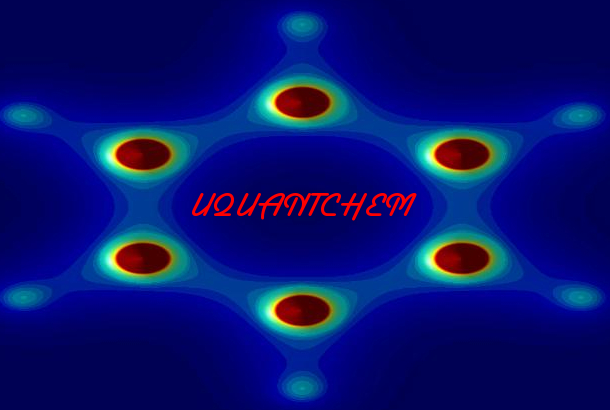
\includegraphics[scale=0.5]{figs/uquantchemLOGO3.jpeg}

\LARGE
\vspace{1cm}
by

Petros Souvatzis

%No Department 

%\vspace{1cm}
%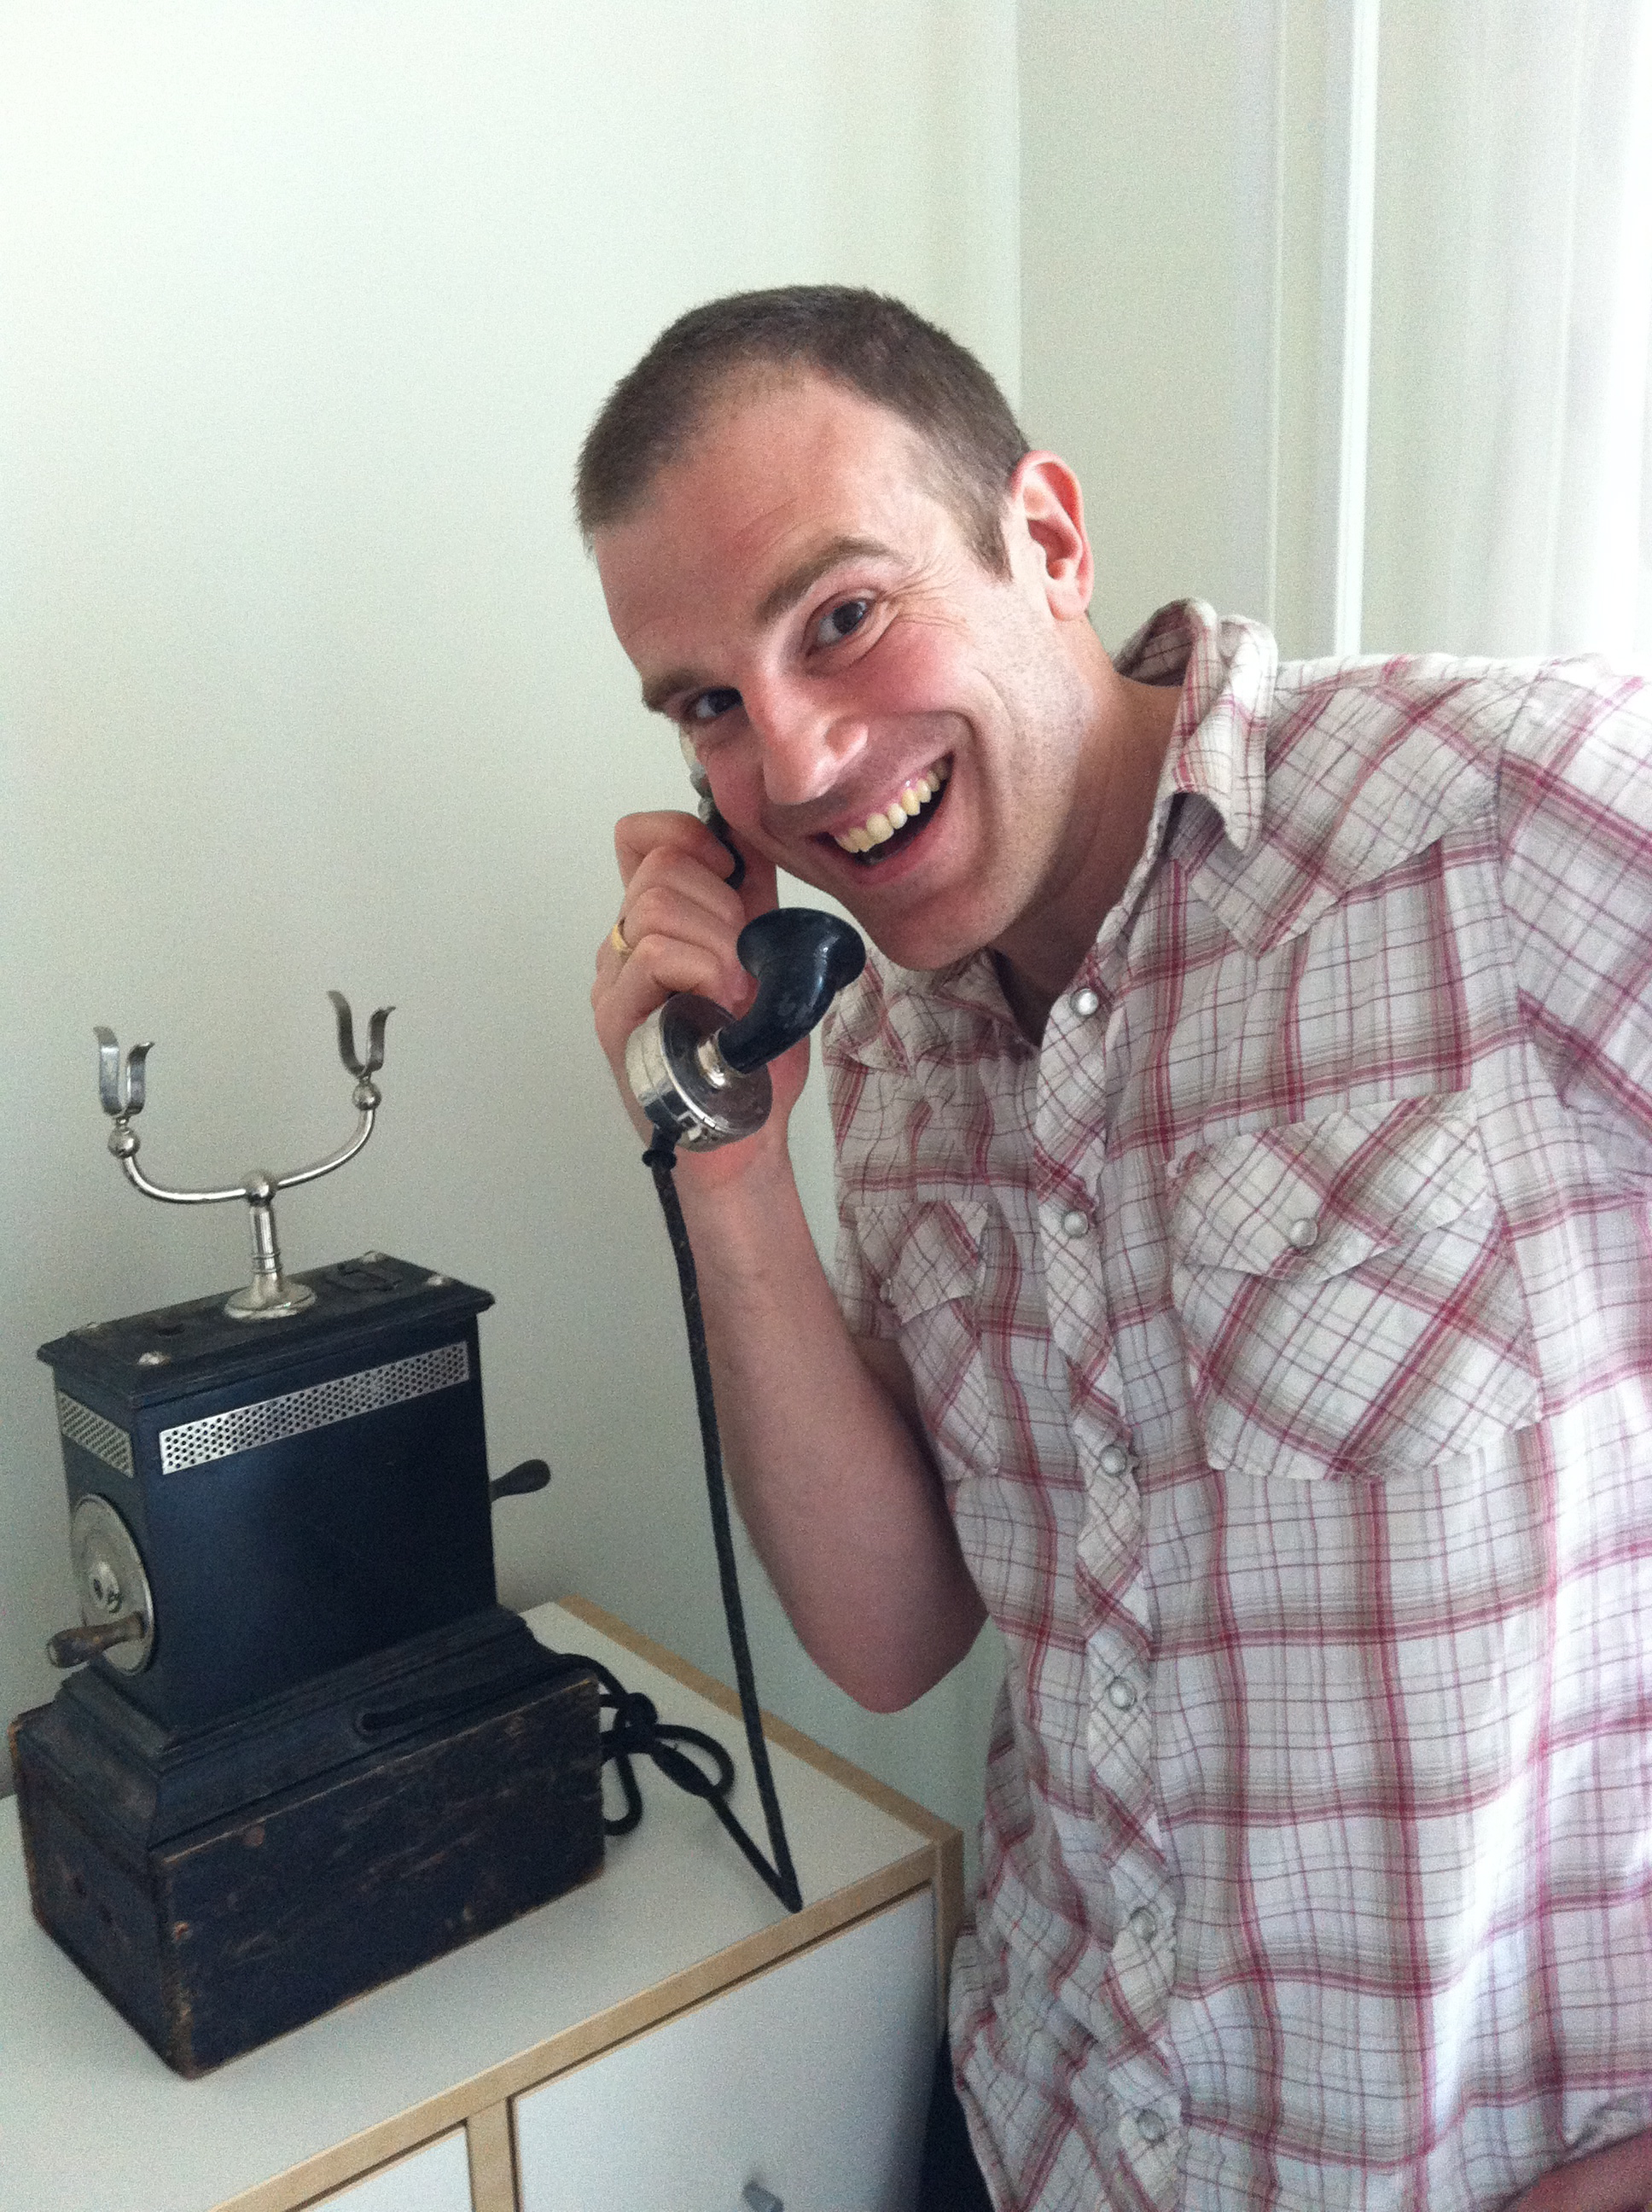
\includegraphics[scale=0.05]{IMG_0083}

Uppsala  2016

\end{centering}
\end{titlepage}

%\newpage

\tableofcontents

\chapter{Introduction}
The Uppsala Quantum Chemistry (UQUANTCHEM) project was started in order to build a transparent, from the point of view of a physicist, development platform for 
implementing new computational and  theoretical  ideas  in quantum chemistry. The package is written in fortran90.

 Due to the ambition of transparency, i.e being able to see the physics in-bedded within  
 the source code, the code might not be as fast as other similar codes. Some of the initial inefficiency as been dealt with by parallelization, which hopefully 
has resulted in a  "proof of principle" level of computational speed, which  will be enough to test new ideas on medium sized molecules.

The ultimate goal is to use the platform of UQUANTCHEM to develop new computational schemes within the context of quantum Monte Carlo. . \\ \\
\noindent
The UQUANTCHEM software is published under the General Public License Version 3.0  (GPLv3.0). Thus any one is free to use the  UQUANTCHEM software.
\\ \\
\noindent
It is my sincere wish that you will enjoy using the UQUANTCHEM package as much as I have enjoyed writing it, and that it might help any freshman to better understand 
the techniques used in modern quantum chemistry. \\ \\
\noindent
Petros Souvatzis



\chapter{Compiling the code}
To compile the code you need to have a fortran compiler installed on your machine together with Lapack. If you don't have Lapack installed the latest 
version of Lapack is provided together with the UQUANTCHEM package. There are several pre-made Make-files provided with the UQUANTCHEM package, which 
can be used as templates to create a Make-file that corresponds to the specifications of your particular system. Here an example of a more or less generic 
installation procedure will be given. 
\\ \\
{\bf ALTERNATIVE 1} Let's assume you have the gfortran compiler available on your system and that you also have lapack and blas preinstalled on your machine. Now assume you want to compile the serial version of the the code,
then follow the following steps: \\  \\
(1) \texttt{V.35> cd SERIALVERSION} \\ \\
(2)  \texttt{V.35/SERIALVERSION> cp Makefile.gfortran.serial Makefile} \\ \\
\noindent
(3) In the \texttt{Makefile},  edit the line:\\ 
\indent
 \texttt{LAPACKPATH = /Users/petros/UQUANTCHEM/Src/V.21/lapack-3.4.0} \\
 \indent
 so it reads: \\
 \indent
 \texttt{LAPACKPATH = Path-where-I-have-my-lapack-lib} \\ \\
\noindent
(4) In the \texttt{Makefile},  edit the line:\\ 
\indent
 \texttt{BLASPATH =/Users/petros/UQUANTCHEM/Src/V.21/BLAS} \\
 \indent
 so it reads: \\
 \indent
 \texttt{BLASPATH = Path-where-I-have-my-blas-lib} \\ \\
\noindent
(5)  \texttt{V.35/SERIALVERSION>  make} \\ \\
\noindent
\noindent
\newpage
\noindent
{\bf ALTERNATIVE 2} Let's assume you have the gfortran compiler available on your system and that you {\it do not} have lapack and blas preinstalled on your machine. Then you can compile the lapack and blas libraries 
that comes with the uqantchem package together with uquantchem by following these steps: \\  \\
(1) \texttt{V.35> cd SERIALVERSION} \\ \\
(2)  \texttt{V.35/SERIALVERSION> cp Makefile.gfortran.nolapack.noblas.serial Makefile} \\ \\
\noindent
(3) In the \texttt{Makefile},  edit the line:\\ 
\indent
 \texttt{LAPACKPATH = /Users/petros/UQUANTCHEM/Src/V.21/lapack-3.4.0} \\
 \indent
 so it reads: \\
 \indent
 \texttt{LAPACKPATH = Where-uquantchem-is-located-on-my-machine/lapack-3.4.0} \\ \\
\noindent
(4) In the \texttt{Makefile},  edit the line:\\ 
\indent
 \texttt{BLASPATH =/Users/petros/UQUANTCHEM/Src/V.21/BLAS} \\
 \indent
 so it reads: \\
 \indent
 \texttt{BLASPATH = Where-uquantchem-is-located-on-my-machine/BLAS} \\ \\
\noindent
(5)  \texttt{V.35/SERIALVERSION>  make all} \\ \\
\noindent
\noindent

And similarly if you want to install the openmp or the MPI-version of  the code you do just move in to the  \texttt{OPENMPVERSION}-directory  or the \texttt{MPI\_VERSION}
-directory and perform the steps (2)-(5). In the case of the openmp/gfortran version the simplest way to install is to use the pre-made make-file named \texttt{Makefile.gfortran.openmp}, 
or if you have access to any of the Swedish super-computer clusters Lindgren or Neolith there are also pre-made Make files for the MPI-version of the code to make life 
easier.


%===========================^M
\chapter{What Can be done with UQUANTCHEM}
%===========================^M

%%%%%%%%%%%%%%%%%%%
\section{Hartree Fock Calculations}
%%%%%%%%%%%%%%%%%%%
There are to types of Hartree-Fock types of Hartree-Fock implemented in UQUANTCHEM. The restricted Hartree-Fock (RHF), and unrestricted Hartree Fock (URHF). 
The implementation is based on expanding the molecular orbitals of the slater determinant in a basis set consisting of contracted gaussian primitive functions.
The implementation is of text-book style based on the the book of Szabo Ostlund \cite{Szabo} and the book of Cook \cite{Cook}. To calculate the electron electron 
repulsion integrals $(ij|kl)$ rys quadrature is used.

\section{Configurational Interaction Calculations}
Configuration interaction calculations is possible to perform with UQUANTCHEM with a basis set constructed by double and single excitations of the original 
Hartree-Fock slater determinant (CISD). For mor details see Szabo and Ostlund, p. 231-269. \cite{Szabo}.

\section{M\"oller Plesset Calculations (MP2)}
Standard many body perturbation theory calculations up to second order, so called M\"oller Plesset Calculations (MP2), are also possible. 
For more details see Szabo and Ostlund, p. 350-353. \cite{Szabo}.

\section{Density Functional Theory Calculations (DFT))}
Density functional theory calculations are possible to perform with UQUANTCHEM. The following functionals are available: LDA, PBE and B3LYP.

\section{Time Dependent Density Functional Theory Calculations (TDDFT))}
It is also possible to perform time dependent density functional calculations by real time propagation of the density matrix, P. Here, the quantum Liouville
equation
\begin{equation}
i\frac{dP}{dt} = [F,P] \qquad,
\end{equation} 
is solved by the following algorithm:
\begin{eqnarray}\label{eq:TDDFT}
P(t+\Delta t ) = e^{-i\int_{t}^{t+\Delta t}F(t)dt }P(t)e^{i\int_{t}^{t+\Delta t}F(t)dt }\approx \qquad \qquad \nonumber \\
 \nonumber \\
e^{-i\frac{\Delta t}{4}[7F(t)-4F(t-\Delta t) + F(t-2\Delta t) ] }P(t)e^{i\frac{\Delta t}{4}[7F(t)-4F(t-\Delta t) + F(t-2\Delta t) ] }
\end{eqnarray}
Here, $F$, is the Kohn-Sham Fockian/Hamiltonian of the system. The much too unstable "modified midpoint algorithm" \cite{midpoint}, is no longer used.

\section{Quantum Montecarlo Calculations }
It is possible to perform two types of quantum Monte Carlo calculations. Variational Monte Carlo (VMC) which is mainly used to generate good initial 
random walker configurations for the Diffusion Quantum Monte Carlo (DQMC) calculations. The implementation of DQMC in UQUANTCHEM follows 
closely the algorithm outlined in the work of Umrigar and Nightingale \cite{UMRIGAR}. However, in UQUANTCHEM the trial function is constructed 
with a much simpler Jastrow factor, $\mathcal{J}$,  and slater determinants are constructed from cusp corrected gaussian orbitals. The implementation of the cusp correction 
in UQUANTCHEM follows that described by S. Manten and A. L\"uchow \cite{CUSP}. \\ \\
\noindent
The explicit form of the trial function used for the importance sampling in the DQMC of UQUANTCHEM is given by:
\begin{equation}
\Psi_{T} = D_{\uparrow}D_{\downarrow}\mathcal{J}.
\end{equation}
Where 
\begin{equation}
\mathcal{J} = exp(\sum_{i<j}\frac{\delta\cdot\texttt{BJASTROW}\cdot r_{ij}}{(1+ \texttt{CJASTROW}\cdot r_{ij})},
\end{equation}
$r_{ij} = | r_{i} - r_{j}|$ is the distance between electron $i$ and $j$, $D_{\uparrow}$ and $D_{\downarrow}$ are the slater determinants created from spin up respectively 
spin down orbitals. The orbitals are constructed from the URHF self consistent solution. Here $\delta = 0.25$ if the spin of the electrons $i$ and $j$ are identical otherwise 
if the spins are opposite $\delta = 0.5$.The jastrow parameters \texttt{BJASTROW} and \texttt{CJASTROW} are described the section below discussing the input parameters.

\section{Born Oppenheimer Molecular Dynamics}
Molecular dynamics calculations can be performed within the computational framework provided by uquantchem. The nuclei are here propagated with Newtons classical 
equations of motion, in the context of  the Born-Oppenheimer approximation. The inter-atomic forces are calculated analytically from the gradients of the Hartree-Fock energy (RHF or URHF)
with respect to the nuclear positions. The extended Lagrangian Molecular Dynamics formalism (XL-BOMD) \cite{AMN1,AMN2,XLBOMD} has been implemented providing a total energy 
almost completely free of drift. Furthermore the Fast First Principles Molecular Dynamics formalism (FFP-MD) has also been implemented providing a very stable time propagation without 
employing self consistency!

\chapter{Setting up a UQANTCHEM calculation}


\section{The input files}
There are only two input files that one needs to provide the UQUANTCHEM code, the \texttt{INPUTFILE}-file contains the required information about which atoms 
are present in the molecule, there positions and  the level of approximation used to deal with the electron correlation. On top of this basic information the user 
can provide more detailed information about convergence criteria and  parameters that deals with other levels of approximation or details about the calculation.
These non-basic parameters have been given more or less reasonable default values so that to enable un experienced users to get up in the "air" quickly without being 
weighted down with to many technical details. \\ \\
The second input file needed is the \texttt{BASISFILE}-file, containing information about the basis set to be used by UQUANTCHEM. More specifically, the \texttt{BASISFILE}-file
contains information about the orbital quantum numbers of the basis functions the gaussian exponents and the contraction coefficients. 


\subsection{The \texttt{INPUTFILE}-file}
In the the  sub-directory  \texttt{V.35/EXAMPLE\_INPUT\_OUTPUT/} several example input-files can be found.
Here we only give an example of a INPUT-file specifying a URHF calculation of a water molecule:\\ \\
\texttt{CORRLEVEL URHF}\\
\texttt{TOL 1.0E-8}\\
\texttt{Ne 10}\\
\texttt{NATOMS 3}\\
\texttt{ATOM 1  0.453548746355979 1.751220869758844 0.0000000}\\
\texttt{ATOM 8  0.000000000000000 0.000000000000000 0.0000000}\\
\texttt{ATOM 1 -1.809000000000000 0.000000000000000 0.0000000}

\subsection{The \texttt{BASISFILE}-file}
In the sub-directory \texttt{V.35/BASIS} several basis files can be found. To use a specific type of gaussian basis set just copy the  file containing 
the basis you want to use in your calculation from the \texttt{V.13/BASIS} directory  to the \texttt{BASISFILE}-file. For example if you want to use 
the $6-31G^{**}$ basis set just type: \\ \\
\noindent
\texttt{cp  ../V.35/BASIS/6-31GST-ST.dat   BASISFILE}.
A word of caution should be said about the \texttt{BASISFILE}-file. {\bf IN ORDER FOR THE CORRECT BASIS TO BE USED FOR A MOLECULE CONSISTING
OF ATOMS WITH ATOMIC NUMBERS $Z_{1}\leq Z_{2}\leq \cdots \leq Z_{n}$, ALL ATOMS WITH ATOMIC NUMBERS UP TO  $Z_{n}$ MUST BE SPECIFIED IN 
THE  \texttt{BASISFILE}-file FOR THE UQUANTCHEM PROGRAM TO WORK CORRECTLY!} \\ \\
\noindent
Unfortunately, the above specification might not always be fulfilled for some combinations of atoms when using some of the  \texttt{BASISFILE}-files stored in 
the \texttt{V.35/BASIS} subdirectory. So take care!. \\ \\
\noindent
If there is a basis not provided with the current UQUANTCHEM distribution you might find it on the basis set cite:  \texttt{https://bse.pnl.gov/bse/portal}. Here 
you can by means of cut and past create more basis set files. This is done by the following procedure: \\ \\
(1) Go to  \texttt{https://bse.pnl.gov/bse/portal} \\ \\
(2) On the leftmost scroll menu there are a plethora of basis sets defined. Scroll down to the basis set you want to use and mark it. \\ \\
(3) On the periodic table in the middle of the page there will now appear orange colorings in the left  bottom corners of the atom for which a basis exists. \\ \\
(4) Mark the atoms for which you want to use the basis \\ \\
(5) Select the turbomole format and click on the bottom marked "Get Basis Set". \\ \\
(6) Now there will appear a window containing the basis set information you require. Copy this and past it into a file \texttt{BASNAME.raw} located 
in the same directory as the perl-script \texttt{rawtofortranformat.pl} (located in the the sub-directory \texttt{V.35/BASIS}  ) \\ \\
(7) replace the third line in the perl-script reading \texttt{\$header = "aug-pcS-4";} \\ with  \texttt{\$header = "BASNAME";}. \\ \\
(8) run:  \texttt{./rawtofortranformat.pl} and the file \texttt{BASNAME.dat} will be created. This new file 
can be used by UQUANTCHEM.
\newpage
\subsection{The \texttt{BASISFILEAUX}-file}
This file contains the auxiliary basis-set. One can use either the coulomb-fitting basis-set by Weigend \cite{Weigend}, by copying the file 
\texttt{V.35/BASIS/Weigend-Coulomb-Fitting.dat} to the \texttt{BASISFILEAUX}, or the coulomb-fitting basis by Ahlrichs \cite{Ahlrichs1,Ahlrichs2}, by copying the file \texttt{V.35/BASIS} \texttt{/Ahlrichs-Coulumb-fitting.dat}  to \texttt{BASISFILEAUX} . The \texttt{BASISFILEAUX}  is used in the resolution of identity (RI) approximation of the electron repulsion integrals $(ij|kl)$ and needs to be located in the run-directory. To use the RI-approximation one also needs to set the flag \texttt{RIAPPROX} to .TRUE. in the \texttt{INPUTFILE}. \\ \\
Observe that the the coulomb-fitting basis-set by Weigend \cite{Weigend} has been optimized with respect to the basis-sets in \texttt{V.35/BASIS}
having the prefix \texttt{Def2-}. One can of course combine the Weigend auxiliary basis with other basis-sets, but then the performance cannot be 
guaranteed. \\  \\
Also, observe that all bases in \texttt{Weigend-Coulomb-Fitting.dat} and \\ \texttt{Ahlrichs-Coulumb-fitting.dat} corresponding  atomic number $Z>36$ (Xe), have coulomb-fitting basis-set designed to effective core potentials, DO NOT USE THEM. Instead, if you want to use the RI-approximation for atoms
with $Z>36$ I recommend that you use \texttt{V.35/BASIS/UGBS.dat} as auxiliary basis. The \texttt{UGBS.dat} is not really designed to be a auxiliary basis but since it is so extensive it works fine as a first approximation. \\ \\
Finally, one can also use the the auxiliary basis \texttt{DGA1-DFT-Coulomb-Fitting.dat}, which is exclusively developed for pure DFT calculations such that utilizes the PBE and LDA functionals. There is a corresponding auxiliary basis developed exclusively for the approximation of the exchange contribution from $(ij|kl)$, however this would demand the utilization of two auxiliary basis sets which has not yet been implemented in uquantchem.



\subsection{The \texttt{DENSMATSTARTGUESS.dat}-file}
This is an input-file from which the starting guess to the density matrix of a molecule is generated. This starting guess is used in the self consistent field (SCF) calculations such as, RHF, URHF, and DFT to accelerate and facilitate the convergence of the charge density. The \texttt{DENSMATSTARTGUESS.dat}-file 
is generated by running a series of atomic calculations, one for each and every atomic species in the molecule.


\subsection{The \texttt{MOLDYNRESTART.dat}-file}
In this file contains the information needed to continue a Molecular Dynamics Calculation. The file contains the following information: 1-st line of file contains the time step index (integer), the following 
\texttt{NATOMS} lines contain three columns with the atomic positions corresponding to the time-step index of the first line, the \texttt{NATOMS} lines following the atomic positions contain three columns 
with the velocities of the atoms corresponding to the time-step index of the first line, finally the last \texttt{NATOMS} lines  contain three colums with the interatomic forces of the atoms corresponding to the time-step index of the first line.
IF THE FILE \texttt{MOLDYNRESTART.dat } EXISTS IN THE RUNNING DIRECTORY OF UQUANTCHEM THE CALCULATION WILL BE AUTOMATICALLY CONTINUED. TO RESTART A MOLECULAR 
DYNAMICS CALCULATION FROM SCRATCH BE SURE TO REMOVE THIS FILE FROM THE RUNNING DIRECTORY.

\subsection{The \texttt{INITVELO.dat}-file}
This file, if provided, is used in a Molecular Dynamics Calculation to specify the initial velocities of the atoms. The file should contain three columns and 
\texttt{NATOMS} rows of real numbers specifying the initial velocities of the atoms in $[au]$ . This file is {\bf not} read if the file \texttt{MOLDYNRESTART.dat} is present in the 
running directory.

\subsection{Running Uquantchem}
To run, for instance the serial version of UQUANTCHEM, just simply run the command: \\
\texttt{RUN\_DIR> ./uquantchem.s} \\ \\
in the same directory where the INPUTFILE and BASISFILE are located.



\section{Input parameters}

\subsection{\texttt{CORRLEVEL}}
Type: Character. (Default = None)\\
CORRLEVEL = $\{\texttt{URHF,RHF,CISD,MP2,VMC,DQMC,LDA,PBE,B3LYP}\}$ \\ \\
Used for setting the level of electron correlation employed  in the calculation.  \texttt{URHF} = Un restricted Hartree-Fock, \texttt{RHF}=Restricted Hartree-Fock,
\texttt{CISD}=Configuration Interaction Calculation (singles and Doubles), \texttt{MP2}=M\"oller-Plesset second order perturbation theory, \texttt{VMC}=Variational Monte Carlo,
 \texttt{DQMC}=Quantum Diffusion Monte Carlo, \texttt{LDA}= DFT calculation using the Local Density Approximation (LDA) in the spirit of Vosko Wilk and Nusair \cite{VWN},  \texttt{PBE} = DFT calculations using the gradient corrected 
 functional of Perdew, Burke, and Ernzerhof (PBE) \cite{PBE},   \texttt{B3LYP} = DFT \cite{VWN,LYP,BECKE88,B3LYP} calculations using the hybrid functional of B3LYP.
 
 
  \subsection{\texttt{ADEF}}
Type: Logical. (Default = .FALSE.)\\
If true then all the time independent calculations will be performed with a static field present. In the case of a molecular dynamics calculation, depenpending on 
the parameter \texttt{EPROFILE},  the field will have different time evolutions during the  molecular dynamics run (see section below describing \texttt{EPROFILE}). The option \texttt{EPROFILE=DP} does not work when \texttt{ADEF=.TRUE.}. There is also
an extra option for \texttt{EPROFILE} (not available when when \texttt{DOTDFT=.TRUE.} , i.e for TDDFT/THF calculations), and that is \texttt{EPROFILE='ST'}, which will result in all calculations being perfomed in the presence of a static electric 
field of strength \texttt{EFIELDMAX}. \\ 

When doing molecular dynamics calculations in the presence of a time-dependent external electric field, the electrons are assumed to follow the field adiabatically. Therefore great care should 
be taken to make sure that the system evolves as closely as possible to the ground state of the system. The validity of the adiabatic approximation might be evaluated by calculating the occupation numbers for the hartree-fock/Kohn-Sham orbitals
as a function of time by performing a TDDFT/THF calculation with the same field that is going to be used in the MD-run. If the fluctuations of the orbital occupation numbers are not to severe the adiabatic approximation can be used at least 
with some confidence.
 
 \subsection{\texttt{DOTDFT}}
 Type: Logical. (Default = .FALSE.)\\
 If true, then a time dependent density functional calculation (TDDFT) is performed if \texttt{CORRLEVEL}= $\{\texttt{LDA,PBE,B3LYP}\}$, otherwise if \texttt{CORRLEVEL}= $\texttt{URHF}$, 
 then a time dependent Hartree-Fock calculation is performed. This has only been implemented in the MPI and OPENMP version of the code.


\subsection{\texttt{NSCCORR}} 
Type: Integer. (Default = 0)\\
If \texttt{NSCCORR}$>$0, this integer equals the maximum number of self consistent correction iterations is to be performed after the TDDFT propagation 
$P(t) \rightarrow P(t+\Delta t)$ has been executed according to Eqn. (\ref{eq:TDDFT}). This correction is performed by solving the following equation
self consistently for $P(t+\Delta t)$:
\begin{eqnarray}\label{eq:tdftcorr}
P(t+\Delta t) = e^{-i\int_{t}^{t+\Delta t}F(t)dt}P(t)e^{i\int_{t}^{t+\Delta t}F(t)dt} \qquad \Rightarrow \nonumber \\
\nonumber \\
P(t+\Delta t) \approx e^{-i\frac{\Delta t}{2}(F[P(t)]+F[P(t+\Delta t)])}P(t)e^{i\frac{\Delta t}{2}(F[P(t)]+F[P(t+\Delta t)])}
\end{eqnarray}
Here the trapezoid approximation has been used for the integrals. This correction is almost absolutely necessary for all TDDFT calculations in order to maintain stability. The only time one can ignore this correction is for TDHF calculations, i.e if \texttt{CORRLEVEL = URHF,RHF}.

\subsection{\texttt{SCERR}} 
Type: Double precision. (Default = 0.1E-10)\\
The convergence criterion used for the iterative solution of Eqn. (\ref{eq:tdftcorr}).
 \subsection{\texttt{MIXTDDFT}} 
Type: Double precision. (Default = 0.5)\\
The linear mixing used in the iterative solution of  Eqn. (\ref{eq:tdftcorr}).

 \subsection{\texttt{EPROFILE}}
 Type: Character. (Default = 'HO')\\
 Defines weather or not the electric field used in a TDDFT/TDHF calculation is homogeneous or not and the modulation, $\epsilon(t)$, of the field. If  the \texttt{EPROFILE='HO'} then the amplitude of the electric field is defined by
 $E(t, \mathbf{r}) = \epsilon(t)sin(\omega t)$ or if  \texttt{EPROFILE='AC'} then the electric field is defined by  $E(t,\mathbf{r}) = \epsilon(t)sin[\omega t + (c/\omega)\hat{n}\cdot\mathbf{r}]$, where the modulation, $\epsilon(t)$, is defined by:
 \begin{eqnarray}
 \epsilon(t) =  \texttt{EFIELDMAX}\cdot\Big (\frac{\omega t}{2\pi}\Big ) \quad if \quad t < \frac{2\pi}{\omega} \nonumber \qquad \qquad \qquad  \qquad  \qquad  \qquad   \qquad  \qquad \qquad  \qquad   \qquad   \quad \\
 \epsilon(t) = \texttt{EFIELDMAX}  \quad if \quad  \frac{2\pi}{\omega} \nonumber \le t <  (\texttt{NEPERIOD} + 1 )\frac{2\pi}{\omega}   \qquad  \qquad  \qquad  \qquad  \qquad \qquad  \qquad  \qquad \quad \nonumber \\
 \epsilon(t) = \texttt{EFIELDMAX}\cdot( \texttt{NEPERIOD} + 2 - \frac{\omega t}{2\pi}  ) \quad if \quad   (\texttt{NEPERIOD} + 1 )\frac{2\pi}{\omega}  \le t <  (\texttt{NEPERIOD} + 2 )\frac{2\pi}{\omega} \nonumber \\
  \epsilon(t) = 0.0  \quad if \quad t \ge  (\texttt{NEPERIOD} + 2 )\frac{2\pi}{\omega}  \qquad  \qquad  \qquad  \qquad  \qquad  \qquad  \qquad \qquad  \qquad  \qquad   \qquad  \quad \nonumber 
  \end{eqnarray}
 Here $\hat{n}$ is the propagation direction of the Electric field (see \texttt{EDIR} ), and $c$ the speed of light in vacuum. If \texttt{EPROFILE='DP'} the electric field has been assumed to be a Dirac pulse  and equal to 
 \texttt{EFIELDMAX} for $t=0$ (Just at the precise moment when the TDFT/TDHF time propagation starts), and zero for $t> 0$. This modulation is used to calculate absorption spectra since it corresponds to a Dirac perturbation which is a superposition 
 of all frequencies. Here $\omega = \texttt{OMEGA}$. If \texttt{EPROFILE='CIRC'} then the electric-field is circularly polarized and given by 
\begin{equation}
\bar{E}(t,\mathbf{r}) =  \epsilon(t)( \hat{e}_{1}sin[\omega t] + \hat{e}_{2}cos[\omega t] )
\end{equation}
Here if \texttt{EDIR}=1, then $\hat{e}_{1} = \hat{y},\quad \hat{e}_{2} = \hat{z}$,  if \texttt{EDIR}=2, then $\hat{e}_{1} = \hat{z},\quad \hat{e}_{2} = \hat{x}$ and if \texttt{EDIR}=3, then $\hat{e}_{1} = \hat{x},\quad \hat{e}_{2} = \hat{y}$.
 
 \subsection{\texttt{DOABSSPECTRUM}}
 Type: Logical. (Default = .TRUE. if \texttt{INT(TEND/TIMESTEP)} $<$ 10000 otherwise Default = .FALSE.  )\\
 If true, then the Fourier-transform of the dipole moment is calculated and stored to the file \texttt{ABSSPECTRUM.dat }
 
 \subsection{\texttt{NEPERIOD}}
Type: Integer. (Default = 1)\\
Number of periods that the amplitude modulation, $\epsilon(t)$,  is equal to  \texttt{EFIELDMAX}.
 
 \subsection{\texttt{EFIELDMAX}}
 Type: Double. (Default = 0.030 a.u.)\\
 The strength of the electric dipole field used in a TDFT or a TDHF calculation.
 
 \subsection{\texttt{EDIR}}
 Type: Integer (Default = 1)\\
Defines the propagation direction and polarization of the electric dipole field used in a TDFT/THF calculation. If \texttt{EDIR}=1, then the field propagates in the x-direction and is polarized along the y-direction, 
if \texttt{EDIR}=2, then the field propagates in the y-direction and is polarized along the z-direction and if \texttt{EDIR}=3, then the field propagates in the z-direction and is polarized along the x-direction. 
The direction of travel is only important in the case when \texttt{EPROFILE='AC'} (Inhomogeneous fields)  and the wavelength is comparable to the molecule. In the case of \texttt{EPROFILE='DC'} or \texttt{EPROFILE='HO'}
 \texttt{EDIR} only defines the polarization of the Electric field.
\subsection{\texttt{FIELDDIR}}
Type: 3-dim Double array (Default = None)\\
Three-dimensional array defining the polarization of the electric field in an arbitrary direction. Is used in  TDDFT/THF-calculation or ADEF-calculations. If  \texttt{FIELDDIR} is set  it takes precedence over the \texttt{EDIR}-parameter. Observe that this calculation is done by transforming the atomic positions 
into a coordinate system which has its z-axis parallel to the direction of the field polarization, i.e parallel to \texttt{FIELDDIR} = $(E_{x}, E_{y}, E_{z})$. If the field is a time-dependent inhomogeneous-field, \texttt{EPROFILE='AC'}, the field will travel in the y-direction of the new coordinate system. The new coordinate axes $\hat{x}',\hat{y}',\hat{z}'$ are related to the original coordinate system $\hat{x},\hat{y},\hat{z}$ by the following relations:
\begin{eqnarray}
\hat{x}' =  \hat{x}cos(\phi) - \hat{y}sin(\phi) \qquad \qquad \qquad \qquad \quad \quad\nonumber \\
\hat{y}' = \hat{x}cos(\theta)sin(\phi) + \hat{y}cos(\theta)cos(\phi) - \hat{z}sin(\theta)  \nonumber \\
\hat{z}' = \hat{x}sin(\theta)sin(\phi) + \hat{y}sin(\theta)cos(\phi) + \hat{z}cos(\theta)
\end{eqnarray}
where $cos(\theta) = E_{z}/(E_{x}^2+E_{y}^2+E_{z}^2)^{1/2}$, $tan(\phi) = E_{x}/E_{y}$.

  \subsection{\texttt{OMEGA}}
 Type: Double. (Default = 0.076 a.u.)\\
 The frequency of the electric field used in a TDFT or a TDHF calculation if  \texttt{EPROFILE='AC'} or \texttt{EPROFILE='HO'}. The default frequency corresponds to the vacuum wavelength of $\lambda= 600$ nm.
  
 \subsection{\texttt{NCHEBGAUSS}}
 Type: Integer (Default = 100)\\
 The number of radial mesh points used in the Chebushev-Gauss quadrature used to integrate  the exchange correlation energy and exchange correlation potential matrix elements in the radial direction.
 
\subsection{\texttt{RIAPPROX}}
Type: Logical (Default = .FALSE.)
If set to .TRUE. and if the file \texttt{BASISFILEAUX} is present in the run directory, the resolution of the identity \cite{RI1} will be used. This approximation utilizes the auxiliary basis-set to approximate the electron repulsion integrals by:
\begin{equation}
(ij|kl) \approx \sum_{Q,P \in Aux-Bas}(ij|P)(P|Q)^{-1}(Q|kl)
\end{equation}

\subsection{\texttt{LIMPRECALC} (Only openmp-version)}
Type: Integer (Default = 100)\\
The maximum number of basis-functions permitted to be used if all the electron repulsion integrals $(ij|kl)$ (and their derivatives) are to be pre-calculated and stored in the ram memory. If you run out of memory try and set this value lower than the number of basis functions. In the MPI-version all the 
integrals are stored, however since they usually are shared between several nodes the memory problems are not as frequently encountered for multi-node
MPI-calculations. The pre-calculation and storage makes the code at the moment much faster compared to if the integrals where to be assembled  at each 
SCF iteration.

\subsection{\texttt{DIAGDG}}
Type: Logical (Default = .FALSE.) \\
If .TRUE. and if the file \texttt{DENSMATSTARTGUESS.dat} is not present in the run-directory, the following starting guess for the density matrix, $P$, will be 
used:
\begin{equation}
P_{ij} = \frac{N_{e}}{Tr(S)}\delta_{ij}
\end{equation}
$N_{e}$ = total number of electrons in the molecule and, $S$, is the overlap matrix.

 \subsection{\texttt{NLEBEDEV}}
 Type: Integer (Default = 3)\\
 This integer is used to choose the angular mesh employed by the Lebedev quadrature which is used to  integrate  the exchange correlation energy and exchange correlation potential matrix elements in 
 on a spherical surface. The integer and its corresponding number of mesh points are the following: \\
  \texttt{NLEBEDEV=}$\{1,2,3,4,5,6,7,8,9,10,11,12,13,14,15,16,17,18,19,20,21,22,23,24\}$ \\
 $\rightarrow$ \texttt{Number of mesh points = }$\{110,170,194,230,266,302,350,434,590,770,974,1202,$\\
 $ 1454, 1730, 2030, 2354, 2702, 3074, 3470, 3890, 4334, 4802, 5294, 5810\}$. Thus the default number of angular mesh points is 194. \\ 
  
 \subsection{\texttt{MOLDYN}}
Type: Logical (Default = .False.)\\
Flag specifying weather or not to perform a Molecular Dynamics Calculation. If \texttt{MOLDYN= .TRUE.} a Molecular Dynamics Calculation will be performed.

 \subsection{\texttt{DAMPING}}
Type: Double (Default = 0.0)\\
When performing molecular-dynamics it is possible to introduce a phenomenological dynamical friction on the atomic nuclei. The atoms having non-zero
velocities, $\dot{\mathbf{R}}_{i}$ are then subjected to a dynamical friction force, $\mathbf{f}_{i}$ given by
\begin{equation}
\mathbf{f}_{i} = -\texttt{DAMPING}\frac{\mathbf{R}_{i}}{dt}
\end{equation}

 \subsection{\texttt{XLBOMD}}
Type: Logical (Default = .False.)\\
Flag specifying weather or not to perform a Molecular Dynamics Calculation using the time reversible  propagation algorithm by A.M Niklasson
 \cite{AMN1} for updating the density matrix at each time step. If  \texttt{XLBOMD}  is .TRUE. a Molecular Dynamics Calculation using the  A.M Niklasson 
scheme will be performed.

 \subsection{\texttt{SOFTSTART}}
 Type: Logical (Default = .False.)\\
 This flag, if true, specifies the following start up scheme when doing XL-BOMD calculations:\\ \\
(1) FIRST 50 time-steps full scf XL-BOMD with high level (low order) of \\
dissipation, \texttt{DORDER} = 4\\ \\
(2) Next 50 time-steps fast-QMMD still with high level (low order ) of
\\dissipation, \texttt{DORDER} = 4\\ \\
(3) Rest of the calculation is done with XL-BOMD or fast-QMMD together with the 
order of dissipation (\texttt{DORDER}) that has been specified by the user in the INPUTFILE. Here depending on the user input, XL-BOMD or fast-QMMD
is run.


 \subsection{\texttt{DORDER}}
 Type: Integer (Default = 8)\\
 Determines the order of the dissipative force term used in the time propagation of the density matrices \cite{XLBOMD}. The order of the dissipative force equals \texttt{DORDER-1}.
 Is only used if \texttt{XLBOMD} is \texttt{.TRUE.}
 
 \subsection{\texttt{ALPHA}}
 Type: Double Precision (Default = depending on \texttt{DORDER}, see Table I in in \cite{XLBOMD} )\\
 Parameter used in the XLBOMD time propagation of the density matrix. Only used if \texttt{XLBOMD}  is .TRUE.
 
  \subsection{\texttt{KAPPA}}
 Type: Double Precision (Default = depending on \texttt{DORDER}, see Table I in \cite{XLBOMD} )\\
 Parameter used in the XLBOMD time propagation of the density matrix. Only used if \texttt{XLBOMD}  is .TRUE.
 
 \subsection{\texttt{ZEROSCF}}
 Type: Logical (Default = .False.)\\
 If this flag is set to .TRUE. then when performing a Molecular Dynamics Calculation, self consistent calculation to obtain the density matrix is only performed 
 for the initial 10 (first) time steps. This feature is only to be used together with \texttt{XLBOMD} set to .TRUE. since otherwise the density matrix will be constant 
 throughout the MD calculation. The combination of setting both the flags \texttt{ZEROSCF} and \texttt{XLBOMD} equals the method of Fast Quantum Mechanical 
 Molecular Dynamics (FQMMD) as is described by Niklasson et al \cite{AMN2}. 
 
  \subsection{\texttt{ZEROSCFTYPE}}
 Type: Integer (Default = 1) Only available in the OMP and MPI version. \\
 In the case of \texttt{ZEROSCF = .TRUE.} this parameter selects which of two possible energy expressions to use when calculating the total energy and the interatomic 
 forces when performing a molecular dynamics calculation using the XLBOMD scheme with only 1 scf cycle per time step. For simplicity we here assume a non-spin polarized 
 RHF calculation or a non spin-polarized LDA calculation to exemplify the two energy expressions. \\ \\
\noindent
\texttt{ZEROSCFTYPE = 1}\\
$E = 2Tr[hD] + Tr[DG(D)],  \qquad             (RHF)$\\
$E = 2Tr[hD] + Tr[DG(D)] + E_{xc}(D),  \qquad   (LDA)$\\ \\
\noindent
\texttt{ZEROSCFTYPE = 2}\\
$E = 2Tr[hD] + Tr[(2D-P)G( P )],\qquad                 (RHF)$\\
$E = 2Tr[hD] + Tr[(2D-P)G( P )] + E_{xc}(D), \qquad       (LDA)$ \\ \\
\noindent
Here:
$G = \frac{1}{2}[ J - \frac{1}{2}K ]$,  in the case of a RHF calculation and $G = \frac{1}{2}J$,  in the case of a LDA calculation 
P = density matrix propagated by XLBOMD-scheme $D = \Theta[\mu-F[P]]$,     F[P] = Fockian obtained using the density matrix P.
$\Theta$ = step function. $\mu$ = chemical potential, $h =$ one electron hamiltonian and $E_{xc}=$ exchange correlation energy functional.

 \subsection{\texttt{FIXNSCF}}
 Type: Integer (Default = -1)\\
 This is a parameter that if set such that \texttt{FIXNSCF}$>$0, in a molecular dynamics calculation,  the number of scf cycles are kept constant and equal to \texttt{FIXNSCF}.
 However, for the first 10 time steps the total energies are fully converged with respect to the energy tolerance \texttt{TOL}.
 
 \subsection{\texttt{MOVIE}}
Type: Logical (Default = .False.)\\
Flag specifying weather or not to save the atomic positions of every every \texttt{SAMPLERATE}:th time-step in a Molecular Dynamics Calculatio. If set to .TRUE. 
the atomic positions of every  \texttt{SAMPLERATE}:th time-step will be saved to the file \texttt{MOLDYNMOVIE.xsf}.

 \subsection{\texttt{WRITEONFLY}}
Type: Logical (Default = .False.)\\
If true, the total energy, kinetic energy, potential energy and temperature will be written on the screen and into the file "\texttt{MOLDYNENERGY.dat}" during the 
course of a Molecular Dynamics Calculation. If .FALSE. the energies will be saved to the same file in the end of the calculation and no output will be written to 
the screen.

\subsection{\texttt{TEMPERATURE}}
Type: Double Precision. (Default = 300)\\
The temperature used to set the initial velocities in a Molecular Dynamics Calculation. However, if the file \texttt{INITVELO.dat} is present in 
the run directory of the calculation the initial velocities will be set to those velocities specified in the file  \texttt{INITVELO.dat}, and the value 
\texttt{TEMPERATURE} will be ignored.

 \subsection{\texttt{CFORCE}}
Type: Logical (Default = .False.)\\
Flag specifying weather or not to calculate the interatomic forces. If \texttt{CFORCE = .TRUE.} the interatomic forces will be calculated. 
For the interested user, the exchange correlation contribution of the force has been calculated in a similar fashion as described by Johnson {\it et al} \cite{xcforce}

 \subsection{\texttt{PULAY}}
 Type: Integer (Default = 4)\\
 By setting this parameter the user can select between 4 different ways to calculate the Pulay contribution to the interatomic forces. This feature is mainly present 
 to enable  tests  of the numerical stability of the time reversible XLBOMD algorithm. All four different approaches are equivalent and only differ due to numerical 
 noise. If  \texttt{PULAY} is equal to {\bf1} then the following expression is used to calculate the Pulay contribution to the force \cite{f1}:
 \begin{equation}
 F_{Pulay} = 2\sum_{i}\epsilon_{i}C_{i}(\nabla S)C_{i}
 \end{equation}
 If  \texttt{PULAY}  is equal to {\bf2} then the following expression is used to calculate the Pulay contribution to the force:
 \begin{equation}
 F_{Pulay} = 2Tr[ S^{-1}FP\nabla S]
 \end{equation}
  If  \texttt{PULAY}  is equal to {\bf3} then the following expression is used to calculate the Pulay contribution to the force \cite{AMN2}:
   \begin{equation} 
    F_{Pulay} = Tr[  ( S^{-1}FP +  PFS^{-1} )\nabla S]
 \end{equation}
  If  \texttt{PULAY}  is equal to {\bf4} then the following expression is used to calculate the Pulay contribution to the force \cite{f2}:
 \begin{equation}
 F_{Pulay} = 2Tr[ FP(\nabla S)P]
 \end{equation}
 Here, $F$ is the Fockian, $\epsilon_{i}$ and $C_{i}$ are the eigenvalues respectively eigenvectors of the matrix equation $FC_{i}=\epsilon_{i}SC_{i}$, 
 $S$, the overlap matrix and P equals the density matrix:
  \begin{equation}
 P_{\mu\nu} = \sum_{i} C_{\mu i}C_{\nu i}.
  \end{equation}
\subsection{\texttt{TOL}}
Type: Double Precision. (Default = 1.0E-6)\\
Used to set the convergence criterion for the self consistent field calculations, i.e the self consistent Hartree-Fock calculations are terminated when the difference between the total energy 
of two consecutive iterations is  $<$ \texttt{TOL}.

\subsection{\texttt{RELAXN}}
Type: Logical (Default = .False.)\\
Flag specifying weather or not to perform a structure relaxation calculation. If \texttt{RELAXN=.TRUE.} uquantchem performs a structure relaxation calculation.

\subsection{\texttt{RELALGO}}
Type: Integer. (Default = 1)\\
Only used if {\texttt{RELAXN = .TRUE.}. Selects which type of relaxation algorithm to be used when optimizing the atomic positions. If \texttt{RELALGO = 1}, then the optimization 
will be done by searching for the atomic positions for which all the forces are zero. Here caution must be taken since there is no guarantee that the atomic configuration might end 
up in a molecular structure corresponding to a local energy maximum. Thus, even though this is by far the most effective algorithm as compared to \texttt{RELALGO = 2}, always keep 
an eye on the total energy change during the relaxation run. If \texttt{RELALGO = 2}, then the optimization will be done by searching for a minimum of the total energy
with respect to the atomic positions.

\subsection{\texttt{FTOL}}
Type: Double Precision. (Default = 1.0E-4)\\
Used for structure relaxation calculations (\texttt{RELAXN = .TRUE.}). The relaxation of the structure stops when the mean force is   $<$ \texttt{FTOL}, or if the number of relaxation 
moves $>$ \texttt{NSTEPS}. Be careful with using  \texttt{FTOL}$<$1.0E-5, since it might require a huge number of iterations before the structure is relaxed within the prescribed force tolerance.

\subsection{\texttt{NSTEPS}}
Type: Integer. (Default = 500)\\
Used for structure relaxation calculations (\texttt{RELAXN = .TRUE.}). \texttt{NSTEPS} is the maximum number of relaxation moves permitted. 

\subsection{\texttt{DR}}
Type: Double Precision. (Default = 0.5)\\
Only used if {\texttt{RELAXN = .TRUE.}. If \texttt{RELALGO =2} the parameter \texttt{DR} defines the interval $[0,\texttt{DR}]$ along the gradient which the energy is minimized on. Upon this interval the energy 
is calculated at \texttt{NLSPOINTS} number of points and fitted (least squares) to a polynomial of degree \texttt{PORDER-1}.\\
(Only used for structure relaxation calculations \texttt{RELAXN = .TRUE.}). If \texttt{RELALGO =1}, parameter \texttt{DR} is the maximum  distance in au, that the atoms 
are allowed to move in one Newton-Raphson cycle.

\subsection{\texttt{NLSPOINTS}}
Type:  Integer. (Default = 10)\\
Only used if {\texttt{RELAXN = .TRUE.}. Here \texttt{NLSPOINTS}  = number of points in the interval $[0,\texttt{DR}]$ where the energy is sampled. The data $\{DR_{i},E(DR_{i})\}_{i=1}^{\texttt{NLSPOINTS}}$,
is least squares fitted to a polynomial of degree \texttt{PORDER-1}.

\subsection{\texttt{PORDER}}
Type:  Integer. (Default = 7)\\
Only used if {\texttt{RELAXN = .TRUE.}. Here \texttt{PORDER} equals the degree+1 of the polynomial used in the least squares fitting employed in the line-search of the conjugate gradient relaxation of the nuclei.

\subsection{\texttt{MIX}}
Type: Double Precision. (Default = 0.0)\\
Mixing parameter used to linearly mix the density matrix of the previous, $P_{i-1}$, iteration with the density matrix of the current iteration, $P_{i}$, in 
a RHF or a URHF calculation. I.e 
\begin{equation}
P_{i}' = P_{i}(1-\texttt{MIX}) + P_{i-1}\texttt{MIX}
\end{equation}

\subsection{\texttt{ETEMP}  (Only used for \texttt{CORRLEVEL = URHF,LDA,PBE,B3LYP})}
Type: Double Precision. (Default = -1.0) (Only used for \texttt{CORRLEVEL = LDA,PBE,B3LYP})
Electronic temperature used to calculate the electronic free energy in the case of a DFT-calculation and a URHF-calculation. If \texttt{ETEMP}$>$ 0, the density matrix, $P_{\mu\nu}$, will be calculated by occupying the states according to 
Fermi-Dirac statistics, i.e:
\begin{equation}
P_{\mu\nu} =  \sum_{i=1}^{Ne}C_{\mu i}C_{\nu i}^{\dagger} \Big [1 + e^{\beta(\epsilon_{i} - \mu) } \Big ]^{-1}.
\end{equation}
Here $\beta = 1/(K_{B}\texttt{ETEMP})$, $\mu$ is the chemical potential and $\epsilon_{i}$ are the energy eigenvalues of the eigenvalue equation $FC_{i}=\epsilon_{i}SC_{i}$, where $F$ is the Kohn-Sham fockian/hamiltonian.
 Note that if  \texttt{ETEMP}$>$ 0  the parameter $\texttt{PULAY}$ will be automatically set to 2, regardless of 
the specification of  $\texttt{PULAY}$ made in the INPUFILE. The entropy, $\mathcal{S}$, is calculated according to:
\begin{equation}
\mathcal{S} = -K_{B}\sum_{i}\Big [ n_{i}ln(n_{i}) + (1-n_{i})ln(1-n_{i} ) \Big ].
\end{equation}
Where,
\begin{equation}
n_{i} = \Big [1 + e^{\beta(\epsilon_{i} - \mu) } \Big ]^{-1}.
\end{equation}

\subsection{\texttt{DIISORD}}
Type: INTEGER. (Default = 3, ( MAX = 25) )\\
Mixing parameter equal to half of the order of the  direct inversion of  the iterative subspace method (DIIS) \cite{DIIS,DIIS2}. If \texttt{DIISORD}=0 (DEFAULT) the DIIS mixing scheme 
is not used.  The number 2\texttt{DIISORD} equals the number of density matrices mixed together according to:
\begin{equation}
P = \sum_{i=1}^{2\texttt{DIISORD}}\alpha_{i}P_{i}\qquad, \qquad \sum_{i}^{2\texttt{DIISORD}}\alpha_{i}=1.
\end{equation}
such that: $\Delta \mathbf{e'}^{2} = 0$ in the mean square sense, where:
\begin{equation}
\Delta \mathbf{e'} = \sum_{i=1}^{2\texttt{DIISORD}}\alpha_{i}\mathbf{e'}_{i}
\end{equation}
and,
\begin{equation}
\mathbf{e} = FPS-SPF, \qquad \mathbf{e'}=S^{-1/2}\mathbf{e}S^{-1/2}.
\end{equation}
Here F is the Fockian, P the density matrix used to calculate the Fockian F, S the overlap matrix and $S^{-1/2}$ the L\"owdin ortogonalization matrix.
. The index refers to the number of iterations performed 
in the scf cycle. 
 
 \subsection{\texttt{DIISSTART}}
Type: INTEGER. (Default = 50)\\
The DIIS-mixing is used if $\Delta P^{2} < 1$ or until the number of scf iterations $>$ \texttt{DIISSTART}.

\subsection{\texttt{Ne}}
Type: Integer. (Default = Total Nuclear charge of Molecule)\\
Total number of electrons in the molecule.

\subsection{\texttt{NATOMS}}
Type: Integer. (Default = None)\\
Specifies the total number of atoms in the molecule. After this entry there must follow an equal number of rows specifying the atomic species and there 
spatial positions given in cartesian coordinates. The only entries allowed after the \texttt{NATOMS} entry are the rows specifying the atomic species and positions!

\subsection{\texttt{ATOM}}
Type: Integer, Double Precision,  Double Precision,  Double Precision. (Default = None)\\
Four numbers on the same row specifying the atomic number of an atom in the molecule and its corresponding  position in cartesian coordinates. The first number equals the atomic 
number and the three following numbers are the cartesian coordinates, x, y, and z of the atom. 
The entries containing information on the atomic numbers and positions must follow immediately after the \texttt{NATOMS}-entry.

\subsection{\texttt{WRITECICOEF}}
Type: Logical (Default = .False.)\\
Flag specifying weather or not to save the expansion coefficients of the Configuration interaction (CI)  wave function to file or not. If \texttt{WRITECICOEF=.TRUE.} then the CI-wave function 
expansion coefficients are saved to the file \texttt{CIEXPANSIONCOEFF.dat}.

\subsection{\texttt{DIFFDENS}}
Type: Logical (Default = .False.)\\
If true and if \texttt{DOTDFT = .TRUE.} and \texttt{WRITEDENS = .TRUE.}  the differentiated charge density defined by 
\begin{eqnarray}
\Delta \rho^{ex}(\mathbf{r},t_{j}) = \sum_{i=1}^{N_{e}^{\uparrow}}\sum_{\mu,\nu=1}^{N_{B}}(1-n^{\uparrow}_{i})(t_{j})C_{\mu i}^{\uparrow \dagger}(0)C_{\nu i}^{\uparrow}(0)\phi_{\mu}^{\dagger}(\mathbf{r})\phi_{\nu}(\mathbf{r})   \nonumber \\
-\sum_{i=N_{e}^{\uparrow}+1}^{N_{B}}\sum_{\mu,\nu=1}^{N_{B}}n^{\uparrow}_{i}(t_{j})C_{\mu i}^{\uparrow \dagger}(0)C_{\nu i}^{\uparrow}(0)\phi_{\mu}^{\dagger}(\mathbf{r})\phi_{\nu}(\mathbf{r})   \nonumber \\
+\sum_{i=1}^{N_{e}^{\downarrow}}\sum_{\mu,\nu=1}^{N_{B}}(1-n^{\downarrow}_{i})(t_{j})C_{\mu i}^{\downarrow \dagger}(0)C_{\nu i}^{\downarrow}(0)\phi_{\mu}^{\dagger}(\mathbf{r})\phi_{\nu}(\mathbf{r})  \nonumber \\
-\sum_{i=N_{e}^{\downarrow}+1}^{N_{B}}\sum_{\mu,\nu=1}^{N_{B}}n^{\downarrow}_{i}(t_{j})C_{\mu i}^{\downarrow \dagger}(0)C_{\nu i}^{\downarrow}(0)\phi_{\mu}^{\dagger}(\mathbf{r})\phi_{\nu}(\mathbf{r})
\end{eqnarray}
where, $t_{j}$, is given by
\begin{equation}
t_{j} = \frac{j}{24}\texttt{TEND}\quad,j=0,\ldots, 23 
\end{equation}
is written to the files \texttt{DENSEXITED\_0.xsf}, . . . ,\texttt{DENSEXITED\_23.xsf}.

\subsection{\texttt{WRITEDENS}}
Type: Logical (Default = .False.)\\
Flag specifying weather or not to save the charge density to file or not. If \texttt{WRITEDENS =.TRUE.} the the charge density is saved to the file \texttt{CHARGEDENS.dat}. The format of the 
file is the following:  At each row of the file the rightmost number corresponds to the charge density at a spatial point, $r=(x,y,z)$,  specified by the three preceding integers on the same row. These integers,  
lets call them I, J and K, correspond to cartesian coordinates by the following mapping:
\begin{eqnarray}
x(I) = - \texttt{LIMITS(1)}+2\frac{\texttt{LIMITS(1)}(I-1)}{\texttt{MESH(1)}-1} \nonumber \\
y(J) = - \texttt{LIMITS(2)}+2\frac{\texttt{LIMITS(2)}(I-1)}{\texttt{MESH(2)}-1} \nonumber \\
z(K) = - \texttt{LIMITS(3)}+2\frac{\texttt{LIMITS(3)}(I-1)}{\texttt{MESH(3)}-1} \nonumber 
\end{eqnarray}

\subsection{\texttt{MESH}}
Type: Integer, Integer, Integer. (Default = 100 100 100)\\
Specifies the mesh grid to be used when saving the charge density, the homo-density  and the lumo-density to file. For more details on the use of integers in \texttt{MESH} see 
the section about the \texttt{WRITEDENS} parameter.

Also, if \texttt{DOTDFT = .TRUE.}  and if  \texttt{WRITEDENS =.TRUE.} the charge density or differentiated charge density is saved to the files  \texttt{DENSEXITED\_0.xsf}, . . . ,\texttt{DENSEXITED\_23.xsf}.

\subsection{\texttt{LIMITS}}
Type: Double Precision, Double Precision, Double Precision. (Default = 5.0 5.0 5.0)\\
Specifies the the part of space in which the charge density, the homo-density and the lumo-density is to be calculated and saved to file. The part of space in which these densities 
are to be calculated is defined by:
\begin{eqnarray}
x \in [-\texttt{LIMITS(1)},\texttt{LIMITS(1)}] \nonumber \\
y \in [-\texttt{LIMITS(2)},\texttt{LIMITS(2)}] \nonumber \\
z \in [-\texttt{LIMITS(3)},\texttt{LIMITS(3)}] \nonumber 
\end{eqnarray}

\subsection{\texttt{HFORBWRITE}}
Type: Logical (Default = .False.)\\
If true the Hartree-Fock eigen function (orbital) with index \texttt{IOSA} is calculated on the same mesh as defined by \texttt{MESH} and limits defined by \texttt{LIMITS}. The values of the orbital is
saved to the file \texttt{ORBITAL.dat}.

\subsection{\texttt{IOSA}}
Type: INTEGER (Default = (\texttt{Ne}-MOD(\texttt{Ne},2))/2 +MOD(\texttt{Ne},2), THE HOMO-orbital )\\
The index of the orbital which corresponding charge density  being saved to the file  \texttt{ORBITAL.dat} if  \texttt{HFORBWRITE = .TRUE.}

\subsection{\texttt{AORBS}} Type: INTEGER (Default = 0) }\\
If  \texttt{AORBS} $\ne$ 0, this corresponds to the  index of the orbital which is being saved to the file  \texttt{ARBORB.xsf}. If \texttt{AORBS} $>$ 0 the spin-up orbital is saved and
if \texttt{AORBS} $<$ 0 the spin-down orbital is saved. Assuming that the {\it xcrysden} software package have been installed on your machine, you only have to give the following command 
on the command line in order to plot the orbital iso surface: \\ \\
 \texttt{V.35/SERIALVERSION> xcrysden --xsf AORBS.xsf }
 \\ \\
For more details on how to obtain the iso-surface see the section describing the  \texttt{WHOMOLUMO} input flag.

\subsection{\texttt{IORBNR}} Type: INTEGER  (Default = 0) }\\
If  \texttt{IORBNR}$\ne$ 0 then a orthogonality constrained density functional calculation for electronic excited states will be performed according to [J. Phys. Chem. A {\bf 117}, 7378-7392,  (2013)]. The Index of the orbital being excited  and  treated as a hole
is defied by \texttt{IORBNR = 0}. If \texttt{IORBNR = 0}, then no excitation will be performed.
 If \texttt{IORBNR} $>$ 0, then the  spin-up orbital with index $|\texttt{IORBNR}|$ will be treated as a hole, if \texttt{IORBNR} $< $ 0 then the  spin-down orbital with index $|\texttt{IORBNR}|$ will be treated as a hole.


\subsection{\texttt{WHOMOLUMO}}
Type: Logical (Default = .False.)\\
Flag specifying weather or not to save the charge density and the orbital-values of the highest occupied molecular orbital (homo) and the lowest un-occupied molecular orbital (lumo) to  file or not. If \texttt{WHOMOLUMO =.TRUE.} the the charge densities  are saved to the files \texttt{HOMODENS.dat} and \texttt{LUMODENS.dat} and the orbital values are saved to \texttt{HOMO.xsf} and \texttt{LUMO.xsf}. The output format for the \texttt{HOMODENS.dat} is the same as for the  \texttt{CHARGEDENS.dat}-file, 
and the output format of the \texttt{HOMO.xsf} and \texttt{LUMO.xsf} files are that of the {\it xrysden} software package. Assuming that the {\it xcrysden} software package have been installed on your machine, you only have to give the following command 
on the command line in order to plot the HOMO iso surface: \\ \\
 \texttt{V.35/SERIALVERSION> xcrysden --xsf HOMO.xsf }
 \\ \\
 after which  you go to the  \texttt{\underline{T}ools} drag-down menu of the {\it xcrysden} program and select the  "iso-surface" alternative. Then choose the \texttt{Data Grid} alternative, click ok. Finally you fill in 
 your \texttt{Isovalue:} (usually 0.1 is a good default to start with), click the  \texttt{Render +/- isovalue} and click on the  \texttt{Submit} button in the lower right corner of the pop-up menu, and you will have created 
 a isosurface of your HOMO orbital.
 

\subsection{\texttt{APPROXEE}}
Type: Logical (Default = .TRUE.)\\
if \texttt{APPROXEE=.TRUE.} then elements of the four-electron tensor, $(i,j|k,l)$, for which the following condition is satisfied:
\begin{eqnarray}
\sqrt{(i,j|i,j)(k,l|k,l)}P_{max} < \texttt{EETOL} \\
\nonumber \\
P_{max}=Max(2|P_{ij}|, 2|P_{kl}|, |P_{ik}|,|P_{jk}|,|P_{il}|,|P_{jl}|)
\end{eqnarray}
will not be calculated and approximately set to zero. This is to enable a more effective alternative to calculating the electron repulsion tensor $(i,j|k,l)$ between orbitals  that are centered far from 
each other. If \texttt{APPROXEE=.FALSE.} all elements of the tensor will be calculated.

\subsection{\texttt{EETOL}}
Type: Double Precision (Default = 1.0E-10)\\
The threshold used in the approximation of the four-electron tensor, $(i,j|k,l)$. See above definition of \texttt{APPROXEE} for more details.

\subsection{\texttt{BETA}}
Type: Double Precision. (Default = 1.0)\\
Parameter used for updating the total energy estimate, $E_{R}$, used in quantum Monte Carlo calculations. Whenever the time step number, $I$, satisfies $MOD(I, \texttt{NRECALC}) \neq 0$, 
the energy estimate is updated according to
\begin{equation}
E_{R}(I) = \langle E_{R} \rangle_{I-1} +\frac{\texttt{BETA}}{\tau_{eff} \texttt{NRECALC}} log \Big(\frac{\texttt{NREPLICAS}}{W_{I} } \Big)
\end{equation}
here, $I$, is the time step number, $W_{I}$ = Number of replicas of the current  time-step, and \texttt{NRECALC} = Integer number set by the user (Default = $Int(1/ \texttt{TIMESTEP})$ ) which defines the frequency
 in  which the energy update instead is done by  following prescription
 \begin{equation}
E_{R}(I) = \langle E_{L} \rangle_{I-1} + \frac{1}{\tau_{eff} \texttt{NRECALC}} log \Big(\frac{\texttt{NREPLICAS}}{W_{I} } \Big)
\end{equation}
i.e whenever  $MOD(I, \texttt{NRECALC}) = 0$. Here
\begin{equation}
\langle E_{x} \rangle_{n} = \frac{1}{n}\sum_{ j=1}^{n} E_{x}(j), \quad x=L,R, \quad \tau_{eff} = \texttt{TIMESTEP}\frac{N_{a}(I)}{W_{I}}
\end{equation}
Here $N_{a}(I)$ is the number of walkers accepted to move. See for instance Umrigar, {\it et al} \cite{UMRIGAR}.

\subsection{\texttt{NREPLICAS}}
Type: Integer. (Default = 2000)\\
Total number of initial random walkers/replicas used in the Diffusion Monte Carlo calculation.

\subsection{\texttt{SAMPLERATE}}
Type: Integer. (Default = 10)\\
{\bf First use} of this parameter is the sample rate employed  in the variational Monte Carlo calculation used to calculate the initial distribution of random walkers. Since the Metropolis algorithm is 
used for the generation of this initial distribution, only random walkers separated by a number of \texttt{SAMPLERATE}-Metropolis moves are used for the initial distribution.
This is  to avoid that the walkers  are correlated \cite{Koonin}. \\ \\
\noindent
{\bf Second use} of this parameter is to specify how often uquantchem is to save the file \texttt{MOLDYNRESTART.dat}. This file contains the information necessary for a continuation of a
Molecular Dynamics Calculation. The file will be saved every \texttt{SAMPLERATE}:th time step. \\ \\
\noindent
{\bf Third use} of this parameter is to specify the sampling rate of the atomic positions used to create the file \texttt{MOLDYNMOVIE.xsf}, if the flag \texttt{MOVIE} is set to .TRUE. .
The atomic positions of  \texttt{SAMPLERATE}:th time step will be used as a movie frame and saved to the \texttt{MOLDYNMOVIE.xsf} -file. To create at gif-movie you need to use
the program xcrysden in the following way: \texttt{>>xcrysden --xsf  MOLDYNMOVIE.xsf}


\subsection{\texttt{NPERSIST}}
Type: Integer. (Default = 50)\\
NPERSIST is the number of generations a random walker in the diffusion quantum Monte Carlo algorithm is permitted to stay in the same position. If a walker 
stays more than NPERSIST generations in one place the acceptance probability is increased by a factor of
\begin{equation}
1.1^{(N_{g}-\texttt{NPERSIST})}. 
 \end{equation}
Here  $N_{g}$ is the number of generations (time-steps) a walker has been rejected to move. This is to avoid a population catastrophe. For more details see Umrigar {\it et al} \cite{UMRIGAR}.

\subsection{\texttt{NRECALC}}
Type: Integer. (Default = Int(1/\texttt{TIMESTEP}))\\
Integer number deciding how often the mean total energy estimate, $\langle E_{R} \rangle$, should be updated so that the number  of walkers is kept close to the initial 
number of walkers \texttt{NREPLICAS}. See the the description of the related parameter \texttt{BETA} for a more detailed description.

\subsection{\texttt{REDISTRIBUTIONFREQ} (Only used in the MPI-version)}
Type: Integer. (Default = 0)\\
The frequency in which the random walkers in a diffusion Monte Carlo calculation are redistributed evenly over the MPI-threads  (processors). For example 
 \texttt{REDISTRIBUTIONFREQ}=3 results in a redistribution of walkers every third time step. If  \texttt{REDISTRIBUTIONFREQ}=0 then the walkers are redistributed only 
 if there is a threat of all walkers being killed on one computational node (thread/processor) or if there is a risk of overpopulation of walkers at one node. Observe that in order
 to enable a restart of a DQMC calculation one has to set  \texttt{REDISTRIBUTIONFREQ}$>$0. This will force uquantchem to save all the information needed to continue a
 DQMC calculation to the file  \texttt{DQMCRESTART.dat} every \texttt{REDISTRIBUTIONFREQ}:th time-step. If the file  \texttt{DQMCRESTART.dat} exists uquantchem will 
 continue the  DQMC calculation from the time-step at which the file \texttt{DQMCRESTART.dat} was latest updated.

\subsection{\texttt{TEND}}
Type: Double Precision. (Default=10.0)\\
Specifies the run time of the Diffusion Quantum Monte Carlo calculation, aMolecular Dynamics Calculation or a TDDFT calculation.

\subsection{\texttt{TSTART}}
Type: Double Precision. (Default=\texttt{TIMESTEP})\\
Specifies at which time one will start calculating the mean value of the local energy, $E_{L}$, i.e 
\begin{equation}
\langle E_{L} \rangle = \frac{\texttt{TIMESTEP}}{\texttt{TEND}-\texttt{TSTART}}\sum_{t = \texttt{TSTART}}^\texttt{TEND}E_{L}(t)
 \end{equation}

\subsection{\texttt{TIMESTEP}}
Type: Double Precision. (Default=0.0025)\\
Specifies the time-step of the Diffusion Quantum Monte Carlo calculation, a Molecular Dynamics Calculation or a TDDFT calculation.

\subsection{\texttt{CUTTOFFFACTOR}}
Type: Double Precision. (Default=1.0)\\
Specifies the cut-off for the local energy, $E_{L}$,  in a QDMC calculation. Is used to discard pathological configurations. If the the positions of 
a walker generation, $I$, generates a local energy, $E_{L}(I)$, such that 
\begin{equation}
\frac{E_{R}-E_{L}(I)}{|E_{R}|} > CUTTOFFFACTOR
\end{equation}

\subsection{\texttt{CUSPCORR}}
Type:  LOGICAL. (Default= .TRUE.)\\
If  \texttt{CUSPCORR}=\texttt{.TRUE.} then the basis functions are corrected so that they have the correct nuclear cusp behavior close to the nuclei. 
This correction is done in the spirit of S. Manten {\it et al} \cite{CUSP}. This correction is only used for quantum Monte Carlo calculations.

\subsection{\texttt{rc}}
Type: Double Precision. (Default=0.10)\\
If nuclear cusp correction is used the basis functions are corrected  at distances $\leq$ \texttt{rc} from the nuclei at which they are centered.

\subsection{\texttt{CORRALCUSP}}
Type:  LOGICAL. (Default= .TRUE.)\\
If true all basis functions will be cusp corrected. If false only basis functions constructed from contractions of more than 1 primitive gaussiam will be cusp corrected.

\subsection{\texttt{BJASTROW}}
Type: Double Precision. (Default=1.0)\\
Parameter used in the Jastrow factor, $\mathcal{J}$, containing the explicit electron correlation in the trial function
\begin{equation}
\Psi_{T} = D_{\uparrow}D_{\downarrow}\mathcal{J}.
\end{equation}
Where 
\begin{equation}
\mathcal{J} = exp(\sum_{i<j}\frac{\delta\cdot\texttt{BJASTROW}\cdot r_{ij}}{(1+ \texttt{CJASTROW}\cdot r_{ij})},
\end{equation}
$r_{ij} = | r_{i} - r_{j}|$ is the distance between electron $i$ and $j$, $D_{\uparrow}$ and $D_{\downarrow}$ are the slater determinants created from spin up respectively 
spin down orbitals. The orbitals are constructed from the URHF self consistent solution. Here $\delta = 0.25$ if the spin of the electrons $i$ and $j$ are identical otherwise 
if the spins are opposite $\delta = 0.5$. Observe that \texttt{BJASTROW} should be kept equal to one since this help avoid infinities in the local energy, $E_{L}$, when 
$r_{i}=r_{j}$. Thus the only variational parameter that can be used in variational Monte Carlo Calculations (  \texttt{CORRLEVEL = VMC}) is \texttt{CJASTROW}.

\subsection{\texttt{CJASTROW}}
Type: Double Precision. (Default=0.5)\\
See above description of \texttt{BJASTROW}.

\subsection{\texttt{NVMC}}
Type: INTEGER. (Default = 1000000)\\
Number of Metropolis configurations used in the variational Monte Carlo calculation. Note that there are \texttt{SAMPLERATE} number of metropolis moves in between 
every Metropolis configurations used. Thus there are a total of $\texttt{NVMC}\cdot \texttt{SAMPLERATE}$ Metropolis moves performed.

\subsection{\texttt{LEXCSP}}
Type:  LOGICAL. (Default= .FALSE.)\\
If true the slater determinants used in the configuration interaction calculation (  \texttt{CORRLEVEL  = CISD}) will be limited to the slater determinants created by exchanging the \texttt{NEEXC} highest 
occupied Hartree-Fock orbitals with unoccupied Hartree-Fock orbitals that have energy eigen values $<$ \texttt{ENEXCM}.

\subsection{\texttt{ENEXCM}}
Type: Double Precision. (Default= None)\\
See description of \texttt{LEXCSP}.

\subsection{\texttt{NEEXC}}
Type: INTEGER. (Default = \texttt{Ne}, if  \texttt{LEXCSP=.FALSE.})\\
See description of \texttt{LEXCSP}.

\subsection{\texttt{SPINCONSERVE}}
Type:  LOGICAL. (Default= .TRUE.)\\
If \texttt{SPINCONSERVE=.TRUE.} then the total spin of the system is conserved for all excitations used to create the basis set of slater determinants used in the configuration interaction calculations (CISD)
or MP2 calculations. if \texttt{SPINCONSERVE=.FALSE.} then spin-flips will be allowed and the spin of the system is not conserved when creating the CISD basis set or calculating the MP2 correctons.

\subsection{\texttt{RESTRICT}}
Type:  LOGICAL. (Default= .FALSE.)\\
If true then the CISD and MP2 calculations will be based un slater determinants created from a restricted Hartree-Fock (RHF) calculation.

\section{The output files}

\subsection{The \texttt{CHARGEDENS.dat}-file}
In this file the charge density calculated with Hartree-Fock or Diffusion Quantum Monte Carlo is saved. The file consists of four columns. The first three columns (counting from left to right) 
contain integer numbers corresponding to the coordinate mesh indexes $I,J,K$ described together with the input parameters \texttt{WRITEDENS} and \texttt{MESH}. The fourth column 
contains the calculated values of the charge density $\rho(x(I),y(J),z(K)) = \rho(x,y,x)$.

\subsection{The \texttt{RHFEIGENVALUES.dat}-file}
In this file the energy eigenvalues of the  restricted  Hartree-Fock  calculation (RHF) are stored. First column eigenvalue index and second column eigenvalues. 
of the spin down orbitals.

\subsection{The \texttt{UHFEIGENVALUES.dat}-file}
In this file the energy eigenvalues of the  unrestricted Hartree-Fock  calculation (URHF) are stored. First column eigenvalue index, second column eigenvalue of spin up orbitals and third column eigenvalues 
of the spin down orbitals.

\subsection{The \texttt{ORBITAL.dat}-file}
In this file the  Hartree-Fock eigen function, $\Psi_{\texttt{IOSA}}$, calculated on the mesh specified by  the input parameters \texttt{WRITEDENS} and \texttt{MESH} is saved. 
The file consists of Five columns. The first three columns (counting from left to right) 
contain integer numbers corresponding to the coordinate mesh indexes $I,J,K$ described together with the input parameters \texttt{WRITEDENS} and \texttt{MESH}. The fourth column 
contains the calculated values of the Hartree-Fock eigen function, $\Psi_{\texttt{IOSA}\uparrow}(x(I),y(J),z(K)) = \Psi_{\texttt{IOSA}\uparrow}(x,y,x)$, and the fifth column contains the 
calculated values of the Hartree-Fock eigen function, $\Psi_{\texttt{IOSA}\downarrow}(x(I),y(J),z(K)) = \Psi_{\texttt{IOSA}\downarrow}(x,y,x)$.

\subsection{The \texttt{ABSSPECTRUM.dat}-file}
Is produced if  \texttt{DOABSSPECTRUM = .TRUE.} or if \texttt{DOABSSPECTRUM} is not explicitly set by the user and \texttt{INT(TEND/TIMESTEP)} $<$ 10000 then the \texttt{ABSSPECTRUM.dat}-file is produced which contains the absorption spectrum, i.e, the time-Fourier transform of the dipole moment, 
\begin{equation}
\mu_{p}(t) = \sum_{atom}(\mathbf{R}_{atom}\cdot\hat{p})Z_{atom}-Tr[P(t)d_{p}].
\end{equation}
Here $\hat{p}$ is the polarization direction 
of the electric field, $P$, the density matrix and, $d_{p}$, the dipole tensor in the polarization direction.

\subsection{The \texttt{TDFTOUT.dat}-file}
Contains information from the TDDFT/TDHF  calculation. First column = time-step index, second column = time, third column = dipole moment, fourth column = expectation value of the effective hamiltonian/Fockian, 
fifth column = total electron  charge, sixth column = electric field.

\subsection{The \texttt{OCCUPATIONUP.dat}-file}
First column contains the time and the second column contains the orbital occupation numbers, $n_{i}(t)$ of the spin-up orbitals, 
\begin{equation}
n^{\uparrow}_{i}(t) = C_{i}^{\uparrow \dagger}(0)P(t)C_{i}^{\uparrow}(0)
\end{equation}
projected out from the density matrix, $P(t)$ of a TDDFT/TDHF calculation.

\subsection{The \texttt{OCCUPATIONDOWN.dat}-file}
First column contains the time and the second column contains the orbital occupation numbers, $n_{i}(t)$ of the spin-down orbitals, 
\begin{equation}
n^{\downarrow }_{i}(t) = C_{i}^{\downarrow \dagger}(0)P(t)C_{i}^{\downarrow}(0)
\end{equation}
projected out from the density matrix, $P(t)$ of a TDDFT/TDHF calculation.

\subsection{The \texttt{DENSEXITED\_0.xsf}, . . . ,\texttt{DENSEXITED\_23.xsf}-files}
If a TDDFT or a TDHF calculation is done and \texttt{WRITEDENS = .T.} and  \texttt{DIFFDENS=.FALSE.} these 24 files containing  the charge density of the excited, $\rho^{ex}(\mathbf{r},t)$, states calculated from the occupation numbers, $n^{\uparrow}_{i}(t) = C_{i}^{\uparrow \dagger}(0)P(t)C_{i}^{\uparrow}(0)$ and $n^{\downarrow }_{i}(t) = C_{i}^{\downarrow \dagger}(0)P(t)C_{i}^{\downarrow}(0)$, are produced. The excited states charge density is given by 
\begin{eqnarray}
\rho^{ex}(\mathbf{r},t_{j}) = \sum_{i=1}^{N_{B}}\sum_{\mu,\nu=1}^{N_{B}}n^{\uparrow}_{i}(t_{j})C_{\mu i}^{\uparrow \dagger}(0)C_{\nu i}^{\uparrow}(0)\phi_{\mu}^{\dagger}(\mathbf{r})\phi_{\nu}(\mathbf{r}) +  \nonumber \\
\sum_{i=1}^{N_{B}}\sum_{\mu,\nu=1}^{N_{B}}n^{\downarrow}_{i}(t_{j})C_{\mu i}^{\downarrow \dagger}(0)C_{\nu i}^{\downarrow}(0)\phi_{\mu}^{\dagger}(\mathbf{r})\phi_{\nu}(\mathbf{r})
\end{eqnarray}
where, $t_{j}$, is given by
\begin{equation}
t_{j} = \frac{j}{24}\texttt{TEND}\quad,j=0,\ldots, 23 
\end{equation}
If however \texttt{DIFFDENS=.TRUE.} then the differentiated charge density defined by 
\begin{eqnarray}
\Delta \rho^{ex}(\mathbf{r},t_{j}) = \sum_{i=1}^{N_{e}^{\uparrow}}\sum_{\mu,\nu=1}^{N_{B}}(1-n^{\uparrow}_{i})(t_{j})C_{\mu i}^{\uparrow \dagger}(0)C_{\nu i}^{\uparrow}(0)\phi_{\mu}^{\dagger}(\mathbf{r})\phi_{\nu}(\mathbf{r})   \nonumber \\
-\sum_{i=N_{e}^{\uparrow}+1}^{N_{B}}\sum_{\mu,\nu=1}^{N_{B}}n^{\uparrow}_{i}(t_{j})C_{\mu i}^{\uparrow \dagger}(0)C_{\nu i}^{\uparrow}(0)\phi_{\mu}^{\dagger}(\mathbf{r})\phi_{\nu}(\mathbf{r})   \nonumber \\
+\sum_{i=1}^{N_{e}^{\downarrow}}\sum_{\mu,\nu=1}^{N_{B}}(1-n^{\downarrow}_{i})(t_{j})C_{\mu i}^{\downarrow \dagger}(0)C_{\nu i}^{\downarrow}(0)\phi_{\mu}^{\dagger}(\mathbf{r})\phi_{\nu}(\mathbf{r})  \nonumber \\
-\sum_{i=N_{e}^{\downarrow}+1}^{N_{B}}\sum_{\mu,\nu=1}^{N_{B}}n^{\downarrow}_{i}(t_{j})C_{\mu i}^{\downarrow \dagger}(0)C_{\nu i}^{\downarrow}(0)\phi_{\mu}^{\dagger}(\mathbf{r})\phi_{\nu}(\mathbf{r})
\end{eqnarray}
is written to the files. The density (or differentiated charge density) is calculated on a mesh defined by the input-parameters: \texttt{MESH} and \texttt{LIMITS}, and saved in the \texttt{.xsf}-format so that they can be utilized by the XcrySden program.

\subsection{The \texttt{HOMODENS.dat}-file}
In this file the charge density corresponding to the highest occupied molecular orbital (HOMO) calculated with Hartree-Fock is saved . The file consists of four columns. The first three columns (counting from left to right) 
contain integer numbers corresponding to the coordinate mesh indexes $I,J,K$ described together with the input parameters \texttt{WRITEDENS} and \texttt{MESH}. The fourth column 
contains the calculated values of the charge density \\ $\rho_{HOMO}(x(I),y(J),z(K)) = \rho_{HOMO}(x,y,x)$

\subsection{The \texttt{LUMODENS.dat}-file}
In this file the charge density corresponding to the lowest  unoccupied molecular orbital (LUMO) calculated with Hartree-Fock is saved . The file consists of four columns. The first three columns (counting from left to right) 
contain integer numbers corresponding to the coordinate mesh indexes $I,J,K$ described together with the input parameters \texttt{WRITEDENS} and \texttt{MESH}. The fourth column 
contains the calculated values of the charge density \\ $\rho_{LUMO}(x(I),y(J),z(K)) = \rho_{LUMO}(x,y,x)$

\subsection{The \texttt{ENERGYDQMC.dat}-file} 
In this file the time step index ( first column) the mean value of the local energy, $\langle E_{L} \rangle$, (second column), the estimate of the ground state energy, $E_{R}$, (third column) and the number 
of random walkers (fourth column) of the Diffusion Quantum Monte Carlo (DQMC) calculation are printed. \\ \\
\noindent
 Don't forget to check the resulting DQMC energy by running the utility program \texttt{dqmc\_check.pl}.
This program (located at \texttt{V.35/UTILITYPROGRAMS}) takes the \texttt{ENERGYDQMC.dat}-file as input and checks the correlation between walker populations separated by \texttt{\$m} time-steps (  \texttt{\$m} = 5 default, and is set by editing the perl script \texttt{dqmc\_check.pl}). The \texttt{dqmc\_check.pl} script will also calculate the mean value of the local energies  $E_{L}$ separated by \texttt{\$m} time-steps.
Remember that uquantchem has no offset when sampling the local energy, $E_{L}$, i.e  \texttt{\$m} = 1. Thus the mean value for the local energy $\langle E_{L}\rangle$, given as output directly from uquantchem, might very well have been calculated 
over correlated populations.

\subsection{The \texttt{DQMCRESTART.dat }-file}
In this file all the information needed to restart a DQMC calculation is stored. If this file is present in the running directory of uquantchem, then the DQMC  calculation will be continued from the time-step 
where the \texttt{DQMCRESTART.dat }-file was most recently updated. Observe that the condition \texttt{REDISTRIBUTIONFREQ} $>$ 0 must be satisfied  in order for the \texttt{DQMCRESTART.dat }
to be created. The \texttt{DQMCRESTART.dat }-file is updated every \texttt{REDISTRIBUTIONFREQ}:th time-step. The possibility to continue a DQMC calculation only exists for the MPI-version of the 
code.

\subsection{The \texttt{MOLDYNENERGY.dat}-file}
The energies and temperature are saved to the file: \texttt{MOLDYNENERGY.dat} ,first column = time step index, second column = total energy,
third column = kinetic energy, fourth column = potential energy, fifth column = temperature and sixth column number of self consistent cycles performed.

\subsection{The \texttt{MOLDYNRESTART.dat}-file}
In this file contains the information needed to continue a Molecular Dynamics Calculation. The file contains the following information: 1-st line of file contains the time step index (integer), the following 
\texttt{NATOMS} lines contain three columns with the atomic positions corresponding to the time-step index of the first line, the \texttt{NATOMS} lines following the atomic positions contain three columns 
with the velocities of the atoms corresponding to the time-step index of the first line, finally the last \texttt{NATOMS} lines  contain three colums with the interatomic forces of the atoms corresponding to the time-step index of the first line.
IF THE FILE \texttt{MOLDYNRESTART.dat } EXISTS IN THE RUNNING DIRECTORY OF UQUANTCHEM THE CALCULATION WILL BE AUTOMATICALLY CONTINUED. TO RESTART A MOLECULAR 
DYNAMICS CALCULATION FROM SCRATCH BE SURE TO REMOVE THIS FILE FROM THE RUNNING DIRECTORY.

\subsection{The \texttt{MOLDYNMOVIE.xsf}-file}
This file contains atomic positions, in $[$\AA$]$, sampled from a Molecular Dynamics Calculation and can be used by the xcrysden program to create a gif-movie of the motion of the molecule. To do this just:
\texttt{>>xcrysden --xsf MOLDYNMOVIE.xsf}, then once xcrysden starts the rest is pretty self explanatory. The resulting movie is most easily viewed by any web browser.


\subsection{The \texttt{ATOMPOSITIONS.dat}-file}
This file contains the latest update of the atomic positions during and after a structural relaxation calculation.

\subsection{The \texttt{HOMO.xsf}-file and the \texttt{LUMO.xsf}-file}
Contain the HOMO and LUMO orbital values  printed on a 3D mesh, and can be used by the xcrysden program to plot iso surfaces of the respective orbitals.


\chapter{Example Calculations}
In the sub-directories \texttt{V.35/EXAMPLE\_INPUT\_OUTPUT/} one can find the results of different uquantchem calculations. \\ \\
 {\bf RUN1}: contains the output and input of a URHF calculation of a water molecule using a $6-31G^{**}$ basis set. \\ \\
\noindent
{\bf RUN2}: contains the output and input of a MP2 calculation of a He atom using a cc-pVQZ basis set. \\ \\
\noindent
{\bf RUN3}: contains the output and input of a CISD calculation of a $H_{2}$ molecule atom using a cc-pVDZ basis set. \\ \\
\noindent
{\bf RUN4}: contains the output and input of a VMC calculation of a $H_{2}$ molecule atom using a $6-31G^{**}$ basis set. \\ \\
\noindent
{\bf RUN5}: contains the output and input of a DQMC calculation of a $H_{2}$ molecule atom using a $6-31G^{**}$ basis set. \\ \\
\noindent
{\bf RUN6}: contains the output and input of a DQMC calculation of a $He$ atom using a cc-pVTZ basis set. \\ \\
\noindent
{\bf RUN7}: contains the output and input of a RHF charge density  calculation for a  $H_{2}O$ molecule  using a $6-31G^{**}$ basis set. \\ \\
\noindent
{\bf RUN8}: contains the output and input of a RHF of a  $Cr$ atom  using a $6-31^{**}$ basis set. Here the one of the d-orbitals  is plotted in the z=0 plane. \\ \\
\noindent
{\bf RUN9}: contains the output and input of a DQMC calculation of a $He$ atom using a cc-pVTZ basis set. Here the calculation is done with 
a slightly smaller time step than in RUN6. Also the charge density has been accumulated from the walker configurations at the different time steps. \\ \\
\noindent
{\bf RUN10}: contains the output and input of a VMC calculation of a $H_{2}O$ using a $6-31G^{**}$ basis set. Also, the charge density has been calculated
from the generated Metropolis configurations.\\ \\
\noindent
{\bf RUN11-20} I have forgotten the exact type of calculations performed, but I think most of them are DQMC or VMC calculations. \\ \\
{\bf RUN21}: contains the output and input of a structure relaxation calculation for $CH_{4}$ using URHF and a 3-21G basis set .\\ \\
\noindent
{\bf RUN22,26}: contains the output and input of a structure relaxation calculation for $H_{2}O$ using URHF and a $6-31G^{**}$ basis set .\\ \\
\noindent
{\bf RUN27}: contains the output and input of a structure relaxation calculation for $H_{2}$ using URHF and a cc-pVDZ basis set .\\ \\
\noindent
{\bf RUN31}: contains the output and input of a structure relaxation calculation for $H_{2}O$ using the PBE functional  and a cc-pVTZ basis set .\\ \\
\noindent
{\bf RUN31}: contains the output and input of a structure relaxation calculation for $H_{2}O$ using the B3LYP  functional  and a STO-3G basis set .\\ \\
\noindent
{\bf RUN33X, RUN33Y, RUN33Z}: contains the output and input three TDDFT calculations  for $H_{2}O$ using the PBE  functional  and  the 6-31G  basis set .
See figure \ref{Figure_3} for the resulting absorption spectrum.\\ \\

\begin{figure}[tbp]
\includegraphics*[angle=0,scale=0.5]{TDFT}
\caption{\label{Figure_3}\small
Absorption spectrum calculated with uquantchem's TDDFT  implementation. Here 3 Dirac pulses where used to produce the spectrum. A 6-31G  basis  set 
together with the PBE functional was used.The corresponding input files 
are INPUTFILE.RUN33X, INPUTFILE.RUN33Y and INPUTFILE.RUN33Z.  The time step used was 0.05 a.u.}
\end{figure}

\chapter{Utility Matlab programs for plotting}
In the sub-directory \texttt{V.35/UTILITYPROGRAMS} there are a couple of simple matlab scripts that can help you visualize  charge-densities and atomic orbitals 
calculated with UQUANTCHEM. 
%
\chapter{For the developer}
In this chapter the different subdirectories of the directory \texttt{V.35/} and their respective content will be briefly discussed.
\section{File-map}
The following subdirectories are included in the \texttt{V.35} package:
\subsection{\texttt{BASIS}}
This directory contains the files of all the different gaussian basis-sets that accompany this release of uquantchem. 
\subsection{\texttt{BLAS}}
This directory contains the basic linear algebra sub-programs (BLAS) attached to this release of uquantchem to enable 
the compilation of the code in the event that there is no native BLAS on the machine at which uquantchem is to be installed.
\subsection{\texttt{lapack-3.4.0}}
This directory contains the linear algebra package (LAPACK) attached to this release of uquantchem to enable 
the compilation of the code in the event that there is no native LAPACK on the machine at which uquantchem is to be installed.
\subsection{\texttt{UTILITYPROGRAMS}}
This directory contains a number of utility scripts written in perl or to be used with matlab. Here follows a list of the included programs 
and a short description of how the are utilized: \\ \\
\texttt{velautocorr.pl} \\
This script takes the uquantchem movie-file: \texttt{MOLDYNMOVIE.xsf}  
and calculates the velocity-auto-correlation function. The   
result is saved in the file: \texttt{VELAUTO.dat} and performs the temporal fouriertransform of the very same function and saves it to the files \texttt{SPECTRUM\_THz.dat} and \texttt{SPECTRUM\_cm.dat}  \\ \\
\texttt{velautocorr2.pl} \\
A slightly modified version of \texttt{velautocorr.pl}. \\ \\
\texttt{pdbtoau.pl} \\
For converting the atomic coordinates in pdb-files
to a coordinate file suitable for the uquantchem code. \\ \\
\texttt{dqmc\_check.pl}\\
Calculates the mean local energy $E_{L}$ by using every the local energy at every m:th (integer specified by user inside of script) time-step from the out-put file of a dqmc calculation \texttt{ENERGYDQMC.dat}. It also calculates the correlation function.\\ \\
\texttt{distance.pl}\\
This script takes the uquantchem movie-file: \texttt{MOLDYNMOVIE.xsf}
and calculates the interatomic distance between atom A and B
as a function of time.\\ \\
\texttt{isodens.m}\\
This matlab script uses the out-put file \texttt{CHARGEDENS.dat} to calculate and plot an iso-density surface of the charge density.\\ \\
\texttt{isohomolumo.m}\\
This matlab script uses the out-put files \texttt{LUMODENS.dat} and \texttt{HOMODENS.dat}  to calculate and plot an iso-density surface corresponding to the LUMO and HOMO orbitals. 
\subsection{\texttt{TESTS}}
This subdirectory contains the subdirectories:  \texttt{RUN1, RUN2,} $\ldots$ \texttt{,RUN7} which in turn contains input and output files of seven different test calculations performed with the openmp 
version of the uquantchem code. A more detailed specification of these test calculations can be found in the \texttt{README}-file.
\subsection{\texttt{README}}
This file contains basic information on how to compile the uquantchem code and information on the different test calculations located in the subdirectory \texttt{TESTS}.
\subsection{\texttt{manual.pdf}}
This manual that you are now reading.
\subsection{\texttt{SERIALVERSION}}
This subdirectory contains all the fortran source files (*.f90) of the serial version of the uquantchem code together with different Makefiles. Here follows a complete list of the different fortran source files 
and a short description: \\ \\
\texttt{uquantchem.f90}\\
Main program. \\ \\
\texttt{datatypemodule.f90}\\
Module in which the different datatypes specific to the uquantchem code have been defined. \\ \\
\texttt{exchcorrmodule.f90} \\
Module in which the different exchange correlation functionals have been defined in terms of subroutines and functions.\\ \\
\texttt{random.f90}\\
Module for different random number generators to be used in the diffusion quantum monte Carlo calculations.\\ \\
\texttt{Afunc.f90} \\
This is the function A\_lri(l1,l2,Ax,Bx,Cx,gamma) defined
at the top of page 245 in the Cook Book.\cite{Cook} \\ \\
\texttt{RHF.f90}\\
Subroutine for performing restricted Hartree Fock calculations. \\ \\
\texttt{Fnurec.f90}\\
This subroutine calculates the values F\_nu(X) (see Cook Book p.280 ) \cite{Cook} for nu=0,1,2,...,NUMAX, Through the recursion formula
given on the bottom of p. 280 of the Cook Book. \\ \\
\texttt{Fnu.f90}\\
The function F\_nu(x) described in the Cook Book \cite{Cook}
on pages 244 and 280, is here calculated from 
the Kummer confluent hypergeometric function.
See WIRE's Computational Molecular Science, 2012, {\bf 2}: 290-303 \\ \\
\texttt{CISD.f90}\\
Subroutine for the construction and diagonalization of the configuration interaction Hamiltonian constructed from  singles and doubles excitations. \\ \\
\texttt{getK.f90}\\
Subroutine calculating the the exchange matrix $K_{il}$ by contracting  the electron-electron integrals $(ij|kl)$ with the density matrix $P_{jk}$. \\ \\
\texttt{getKv.f90}\\
Vectorized version of \texttt{getK.f90}. \\ \\
\texttt{getJ.f90}\\
Subroutine calculating the the Hartree matrix $J_{ij}$ by contracting  the electron-electron integrals $(ij|kl)$ with the density matrix $P_{kl}$. \\ \\
\texttt{getJv.f90}\\
Vectorized version of \texttt{getJ.f90}. 
\newpage
\noindent
\texttt{gammaf.f90}\\
calculates the value of the GAMMA-function $\Gamma(I+0.5)$
gfortan has the gamma function as an intrinsic function 
whereas ifort on osx does not seem to have it.\\ \\
\texttt{fj.f90} \\
The function f\_j(l,m,a,b) on page 237 in the Cook book \cite{Cook}. \\ \\
\texttt{fac.f90}\\
simple factorial function: n! \\ \\
\texttt{gto.f90}\\
Calculates the value at argument for a spherically symmetric gto
basis function consisting of contracted primitive gaussians. \\ \\
\texttt{gtop.f90}\\
Calculates the radial derivative, at argument r, of a spherically symmetric
gto  basis function consisting of contracted primitive gaussians. \\ \\
\texttt{gtopp.f90}\\
Calculates the second radial derivative, at argument r, of a spherically
symmetric gto basis function consisting of contracted primitive gaussians. \\ \\
\texttt{gtoppp.f90}\\
Calculates the third radial derivative, at argument r, of a spherically
symmetric gto basis function consisting of contracted primitive gaussians. \\ \\
\texttt{eeints.f90}\\
Subroutine that calculates the electron-electron integrals $(ij|kl)$ by Rys quadrature. \\ \\
\texttt{diaghHF.f90} \\
Subroutine that calculates the eigenvalues, $\epsilon$, and eigenvectors, $C$, to the eigenvalue problem: $FC=\epsilon SC$. Here, $F$, corresponds to the 
Fockian matrix and $S$ the overlap matrix.\\ \\
\texttt{diagh.f90} \\
Subroutine that calculates the eigenvalues, $\epsilon$, and eigenvectors, $C$, to the eigenvalue problem: $HC=\epsilon C$. Here, $H$, typically corresponds to the 
Hamiltonian matrix. \\ \\
\texttt{dfac.f90}\\
Function that calculates the double factorial, n!!. \\ \\
\texttt{checkinputfile.f90}\\
This subroutine checks wheater or not the file 'INPUTFILE'
exists and if so, how many lines, NLINES, it contains before the entry of
the number of atoms, NATOMS. \\ \\
\texttt{chargedenssave.f90}\\
This subroutine calculates and  saves  the  charge-density on disk. 
\newpage
\noindent
\texttt{exciteornot.f90}\\
Function used to decide which excitations to use when performing a CISD calculation. \\ \\
\texttt{hforbitalsave.f90}\\
Subroutine that calculates the values of a Hartree-Fock or Kohn-sham orbital on a mesh and saves the result to disk. \\ \\
\texttt{binomfac.f90}\\
calculates the binomial factor
 $ \binom {N} {M}= \frac{N!}{M!(N-M)!}$\\ \\
\texttt{basfunkval.f90}\\
Calculates the value of a real basis-function, $\psi_{i}$, at the spatial
point $r\in\mathbf{R}^3$. I.e, $\psi_{i}( r )$. \\ \\
\texttt{URHF.f90}\\
Subroutine for performing unrestricted Hartree Fock calculations. \\ \\
\texttt{primeeintegral.f90}\\
Function that calculates the electron repulsion integrals $(\mu \nu | \kappa \lambda )$ over the primitive 
gaussian functions $\phi_{\mu},\phi_{\nu},\phi_{\kappa},\phi_{\lambda}$, i,e: \\ \\
\begin{equation}
(\mu \nu | \kappa \lambda )=\int d^{3}\mathbf{r}\int d^{3}\mathbf{r}' \frac{\phi_{\mu}( \mathbf{r} ),\phi_{\nu}( \mathbf{r} ),\phi_{\kappa}(\mathbf{r}'),\phi_{\lambda}(\mathbf{r}')}{|\mathbf{r}-\mathbf{r}'|} \nonumber
\end{equation}
 \\ \\
\texttt{potential.f90}\\
Subroutine that calculates the potential matrix, $V_{ij}$, and the nuclear gradients of the potential matrix, $\nabla_{\mathbf{R}}V_{ij}$. Where $V_{ij}$ is defined by \\ \\
\begin{equation}
V_{ij} = -\sum_{k}\int d^{3}\mathbf{r}Z_{k}\frac{\psi_{i}( \mathbf{r} )\psi_{j}( \mathbf{r} )}{|\mathbf{r}-\mathbf{R}_{k}|}. \nonumber
\end{equation}
Here, $\mathbf{R}_{k}$ are the positions of the nuclei in the molecule and $Z_{k}$ are the respective atomic numbers.
\\ \\
\texttt{overlap.f90}\\
Subroutine that calculates the overlap matrix, $S_{ij}$, and the nuclear gradients of the overlap matrix, $\nabla_{\mathbf{R}}S_{ij}$. Where $S_{ij}$ is defined by \\ \\
\begin{equation}
S_{ij} = \int d^{3}\mathbf{r}\psi_{i}( \mathbf{r} )\psi_{j}( \mathbf{r} ). \nonumber
\end{equation}
\\ \\
\texttt{oneint.f90}\\
This function calculates the Ix(ta) term on p. 974 in J. Comp. Chem. {\bf 11}, 972-977 (1990)
which is used to calculate the two electron integrals through Rys-quadrature. \\ \\
\texttt{normalize.f90}\\
This subroutine calculates the normalization constants 
for all of the basis functions. \\ \\
\texttt{ROOTWEIGHT5.f90}\\
Subroutine that calculates the roots and weights of 5:th order Rys polynomials. The calculation is done by 
polynomial fits of pree-calculated roots and weights. The fits are taken from the GAMES-package ( Same as in Pyquante), a very fast process. \\ \\
\texttt{leastsq.f90}\\
Performs a least square fit of the function 
$f(r) = Ae^{-\lambda r} + C$ to the N data points
$r(i) = \frac{rc}{N-1}*(i-1),\quad y(i) = GTO(r(i)),\quad i=1,2,\ldots,N$ \\ \\
\texttt{makedens.f90}\\
Subroutine that calculates the density matrix, $P_{\mu \nu}$, from the eigen-vectors of the Fockian/Khon-Sham Hamiltonian, $C_{i}$, i.e
\begin{equation}
P_{\mu \nu}= \sum_{i=1}^{N_{occ}}C_{\mu i}C_{\nu i}^{\dagger} \nonumber
\end{equation}\\ \\
\texttt{kinetic.f90}\\
Subroutine that calculates the Kinetic energy matrix, $T_{ij}$, and the nuclear gradients of the kinetic energy matrix, $\nabla_{\mathbf{R}}T_{ij}$. Where $S_{ij}$ is defined by \\ \\
\begin{equation}
T_{ij} = -\frac{1}{2}\int d^{3}\mathbf{r}\psi_{i}( \mathbf{r} )\nabla^{2}\psi_{j}( \mathbf{r} ). \nonumber
\end{equation}
\\ \\
\texttt{ijkl.f90}\\
Function that contacts the 4-component index i,j,k,l, used to label the different electron-electron repulsion integrals  $(ij|kl)$, into one single index.\\ \\
\texttt{homolumosave.f90}\\
Subroutine that calculates the densities and orbital values of the HOMO and LUMO orbitals on a mesh and writes the result to the files \texttt{HOMODENS.dat}, \texttt{LUMODENS.dat}, \texttt{HOMO.xsf} and \texttt{LUMO.xsf}. \\ \\
\texttt{gettotalbasis.f90}\\
If the logical input variable COUNTER=.TRUE. , this subroutine calculates the  size of the total basis set from the local basis sets centered  at the different atoms If COUNTER=.FALSE. , this subroutine returns the total basis set. \\ \\
\texttt{rysquad.f}\\
This subroutine calculates the roots and weights of a Rys polynomial of arbitrary order. \\ \\
\newpage
\noindent
\texttt{rho.f90}\\
Function that calculates the charge density, $\rho$,  from the basis functions 
and the density matrix P at one point in space. \\ \\
\texttt{readin.f90}\\
Subroutine that reads the user specified data stored in the file \texttt{INPUTFILE}. \\ \\
\texttt{ROOTWEIGHT4.f90}\\
Subroutine that calculates the roots and weights of 4:th order Rys polynomials. The calculation is done by 
polynomial fits of pree-calculated roots and weights. The fits are taken from the GAMES-package ( Same as in Pyquante), a very fast process. \\ \\
\texttt{interpol.f90}\\
This routine calculates the interpolating 
cubic polynomial linking together the 
second derivative of an sto-type basis function:
$sto''( r ) = A\lambda^{2}e^{-\lambda r}$ at the 
point $r = r_{c}$, and a the second derivative of a 
gto-type basis function: $gto''( r )$ at $r = r_{c} + \delta r$
so that both the second and the third derivative of the polynomial 
matches that sto at $r=r_{c}$ and the gto at $r=r_{c}+\delta r$. This is 
done according to J. Chem. Phys. {\bf 115}, 5362 (2001). \\ \\
\texttt{gradbasfunkval.f90}\\
Subroutine that calculates  the gradient of a real basis-function, $\phi_{\mu}$, at the spatial
point $\mathbf{r}\in\mathbf{R}^{3}$. I.e, the  gradient = $\nabla \phi_{\mu}(\mathbf{r})$. \\ \\
\texttt{laplacebasfunkval.f90}\\
Function that calculates the value of the laplacian  of a real basis-function, $\phi_{\mu}$, at the spatial
point $\mathbf{r}\in\mathbf{R}^{3}$. I.e, the laplacian = $\nabla^{2} \phi_{\mu}(\mathbf{r})$. \\ \\
\texttt{hforbitalval.f90}\\
Function that calculates the value of a Hartree-Fock orbital or a Kohn-Sham orbital at the spatial point $\mathbf{r}\in\mathbf{R}^{3}$, given 
the eigen-vector $C_{i}$.  I.e the value $\Psi_{i}(\mathbf{r})$. \\ \\
\texttt{gradhforbitalval.f90}\\
Subroutine that calculates the gradient  of a Hartree-Fock orbital or a Kohn-Sham orbital at the spatial point $\mathbf{r}\in\mathbf{R}^{3}$, given 
the eigen-vector $C_{i}$.  I.e the gradient = $\nabla \Psi_{i}(\mathbf{r})$. \\ \\
\texttt{laplacehforbitalval.f90}\\
Subroutine that calculates the laplacian  of a Hartree-Fock orbital or a Kohn-Sham orbital at the spatial point $\mathbf{r}\in\mathbf{R}^{3}$, given 
the eigen-vector $C_{i}$.  I.e the laplacian = $\nabla^{2} \Psi_{i}(\mathbf{r})$. \\ \\
\texttt{det.f90} \\
This function calculates the determinant of a NxN matrix $A$, by first transforming it into upper diagonal form. \\ \\
\newpage
\noindent
\texttt{stoexponent.f90}\\
Finds the exponent, $\lambda$, and coeficient, $A$,  of a slater type orbital, $Ae^{-\lambda r}$ 
by fiting it to the gaussian basis function, $gto( r )$, at the inflexion
point $r_{c}$, i.e at the point where $gto'(r_{c}) = min$. The
exponent, $\lambda$, and coeficient, $A$ are calculated from the
continuity conditions:\\
(1)  $gto(r_{c}) = Ae^{-\lambda r_{c}}$\\
(2)  $gto'(r_{c}) = -A\lambda e^{-\lambda r_{c}}$\\
leading to $\lambda = - gto'(r_{c})/gto(r_{c})$, and $A = gto(r_{c})e^{-gto'(r_{c})r_{c}/gto(r_{c})}$ \\ \\
\texttt{slaterdet.f90}\\
This fuction calculates the slater determiant from:\\
(a) N = Total Number of electrons, \\
(b) BAS = Hartree Fock basis \\
(c) C = Fockian eigenvectors, \\
(d) r = positions the electrons 3N-long array \\
(e) UP = .TRUE. Spin up slater determinant is calculated, otherwise spin-down slater determinant is to be calculated. \\
(f) NS = slater determinant dimension. \\ \\
\texttt{gradslaterdet.f90}\\
This subroutine calculates the gradient of a slater determiant, with 
respect to the electron coordinate I, from: \\
(a) N = Total Number of electrons,\\
 (b) BAS = Hartree Fock basis\\
(c) C = Fockian eigenvectors, \\
(d) r = positions the electrons 3N-long array \\ 
(e) UP = .TRUE. if I = spin upp orbital, else UP = .FALSE. \\
(f) NS = Slaterdeterminant dimension \\ \\
\texttt{laplaceslaterdet.f90}\\
This fuction calculates the laplacian of a slater determiant, with 
respect to the electron coordinate I, from: \\
(a) N = Total Number of electrons, \\
(b) BAS = Hartree Fock basis \\
(c) C = Fockian eigenvectors, \\
(d) r = positions the electrons 3N-long array \\
(e) NS = Slaterdeterminant dimension.\\
(f) UP = .TRUE. if I = spin upp orbital, else UP = .FALSE. \\ \\
\texttt{jastrowup.f90}\\
This function calculates the Jastrow factor contribution
from the spin-up electrons. N = total number of electrons
r = coordinates of all electrons, r is a 3*N-long array
b,c = jastrow parameters. \\ \\
\newpage
\noindent
\texttt{jastrowdown.f90}\\
This function calculates the Jastrow factor contribution
from the spin-down electrons. N = total number of electrons
r = coordinates of all electrons, r is a 3*N-long array
b,c = jastrow parameters.  \\ \\
\texttt{jastrowud.f90}\\
This function calculates the Jastrow factor contribution
from the cross-terms between spin-up and spin-down electrons. 
N = total number of electrons  r = coordinates of all electrons, r is a 3*N long-array
b,c = jastrow parameters. \\ \\
\texttt{jastrow.f90}\\
This function calculates the (Total) Jastrow factor.
N = total number of electrons
r = coordinates of all electrons, r is a 3*N-long array
b,c = jastrow parameters.  \\ \\
\texttt{DIIS.f90}\\
This is the direct inversion in the iterative subspace method DIIS,
by P. Puley in CHEM. Phys. Lett. {\bf 73}, 393 (1984). The routine is 
used to estimate the self-consistent density-matrix in the region 
where the density dependence of the energy can be approximated well
up to second order. Also, see T. Halgaker, P. Jorgensen and J. Olsen 
 {\it "Molecular Electronic Structure Theory"} p.460-463 \\ \\
 \texttt{findclosestatom.f90}\\
 Subroutine that finds the atomic nucleus located closest to a particular electron. The motivation for 
 the use of this routine can be found in J. Chem. Phys. {\bf 99} , 2865-2890, (1993). \\ \\
 \texttt{gradjastrow.f90}\\
 This subroutine calculates the gradient of the Jastrow factor,
with respect to the electron coordinate I. \\
N = total number of electrons \\
r = coordinates of all electrons, r is a 3*N-long array \\
b,c = jastrow parameters. \\ \\
\texttt{laplacejastrow.f90}\\
This function calculates the laplacian of the Jastrow factor,
with respect to the electron coordinate I.\\
N = total number of electrons \\
r = coordinates of all electrons, r is a Nx3-array \\
b,c = jastrow parameters. \\ \\
\texttt{guideforce.f90}\\
This subroutine calculates the guiding force used in the
DQMC importance sampling.  \\ \\
\texttt{trialfnk.f90}\\
This function calculates the value of the trial function, used in the
DQMC importance sampling,  at a specific point in the $3N_{e}$ dimensional coordinate space of the electrons. ($N_{e}$=number of electrons) \\ \\  
\texttt{laplacetrialfnk.f90}\\
This function calculates the value of laplacian of the trial function, used in the
DQMC importance sampling,  at a specific point in the $3N_{e}$ dimensional coordinate space of the electrons. ($N_{e}$=number of electrons) \\ \\  
\texttt{EL.f90}\\
This function calculates the Local energy  of the trial function, at a specific point in the $3N_{e}$ dimensional coordinate space of the electrons ($N_{e}$=number of electrons).
 Used in the DQMC importance sampling. \\ \\
 \texttt{dqmc.f90}\\
 This routine performs the diffusion quantum Monte Carlo or the  Variational Quantum Monte Carlo calculations. This is the routine that is at the top of the hierarchy/program-tree, i.e the 
 control routine, of all the quantum Monte Carlo  calculations. \\ \\
 \texttt{preparedifusion.f90}\\
 Subroutine that performs a series of calculations in order to enable a diffusion step in the DQMC calculation. For details see J. Chem. Phys. {\bf 99} , 2865-2890, (1993), and the comments embedded in  the 
 source of this routine. \\ \\
 \texttt{ROOTWEIGHTMAX3.f90}\\
Subroutine that calculates the roots and weights of  Rys polynomials of order $\leq$ 3. The calculation is done by 
polynomial fits of pree-calculated roots and weights. The fits are taken from the GAMES-package ( Same as in Pyquante), a very fast process. \\ \\
\texttt{readbasis.f90}\\
This subroutine reads in the expansion coefficients and exponents of the gaussian basis-set stored in the file \texttt{BASISFILE}.\\ \\
\texttt{primpotential.f90}\\
This function calculates the potential energy integral given on the
bottom of p. 244 in the Cook Book \cite{Cook}. \\ \\
\texttt{primoverlap.f90}\\
This function calculates the overlap integral
$S = S_{x}S_{y}S_{z}$ as given by the expressions 
on the pages 234-238 in the Cook book \cite{Cook}. \\ \\
\texttt{primkinetic.f90} \\
 This function returns the integral
$\langle GTO_{1} | -\frac{1}{2}\nabla^{2} | GTO_{2} \rangle$
as given by the cook Book on pages 234-239 \cite{Cook}. Here $GTO_{i}$ are primitive gaussian functions. \\ \\
\texttt{MP2.f90}\\
Subroutine that performs second order  M\o ller-Plesset calculations. \\ \\
\texttt{gradprimoverlap.f90}\\
This subroutine  calculates the nuclear gradients of the overlap integral
$S = S_{x}S_{y}S_{z}$ as given by the expressions 
on the pages 234-238 in the Cook book \cite{Cook}. \\ \\
\texttt{gradprimkinetic.f90}\\
 This subroutine calculates  the nuclear gradients of the integral
$\langle GTO_{1} | -\frac{1}{2}\nabla^{2} | GTO_{2} \rangle$
as given by the cook Book on pages 234-239 \cite{Cook}. Here $GTO_{i}$ are primitive gaussian functions. \\ \\
\texttt{gradprimpotential.f90}\\
This subroutine  calculates the nuclear gradients of the potential energy integral given on the
bottom of p. 244 in the Cook Book \cite{Cook}. \\ \\
\texttt{gradprimeeintegral.f90}\\
This subroutine calculates the nuclear gradients of the two-electron integral between  primitive gaussians. \\ \\
 \texttt{forces.f90}\\
 This subroutine calculates the interatomic forces on all atoms of the molecule. \\ \\
 \texttt{dAfunc.f90}\\
This  function calculates the derivative of the function $A_{lri}(l_{1},l_{2},A_{x},B_{x},C_{x},\gamma)$ ( defined at the top of page 245 in the Cook Book \cite{Cook}) 
with respect to $C_{x}$. \\ \\
\texttt{relax.f90}\\
This subroutine calculates the atomic positions of the molecule that corresponds to the minimal energy.\\ \\
\texttt{linesearchmin.f90}\\ 
This subroutine fits a number of NPOINTS energies and moves 
to 4:th order polynomial in the interval  $[0,DR]$ and calculates
the position of the minimum of this polynomial in the interval $[0,DR]$. This routine is used by \texttt{relax.f90} in order to find the move involved  a steepest decent or a conjugate gradient 
calculation. \\ \\
\texttt{massa.f90}\\
This function just give the atomic mass as output given
the atomic number as input. The atomic masses have been 
taken from Aschcroft and Mermins {\it "Solid State Physics"}. \\ \\
\texttt{moleculardynamics.f90} \\
Subroutine that performs  molecular dynamics calculations. \\ \\
\texttt{moleculardynamicssoft.f90}\\
Subroutine that performs  molecular dynamics calculations, with a so called soft-start. See, the description of the input parameter \texttt{SOFTSTART}. \\ \\
\texttt{invert.f90}\\
Subroutine that inverts a $N\times N$ real matrix.\\ \\
\texttt{vxc.f90}\\
This subroutine calculates the exchange correlation potential. \\ \\
\texttt{vxcalt.f90} \\
Subroutine not used for the moment. \\ \\
\texttt{dvxc.f90}\\
Subroutine not used for the moment. \\ \\
\texttt{ngbasfunkval.f90} \\
Calculates the value of the gradient of a real basis-function at the spatial
point $\mathbf{r}\in\mathbf{R}^{3}$, with respect to the nuclear coordinates at which the basis
function is centered. \\ \\
\texttt{nggradbasfunkval}\\
Calculates the value of nuclear gradient of the gradient of a real basis-function, $\Psi$, at the spatial
point $\mathbf{r}=(x,y,z)$. I.e, the elements of the tensor = $\nabla_{\mathbf{R}}[\nabla\Psi(\mathbf{r})]$.
The output is stored in the 3x3 matrix nggrad, according to the
following ordering:\\ \\
$nggrad(1,1) = \frac{\partial^2\Psi}{\partial R_{x}\partial x},\quad nggrad(1,2) = \frac{\partial^2\Psi}{\partial R_{y}\partial x},\quad nggrad(1,3) = \frac{\partial^2\Psi}{\partial R_{z}\partial x}$ \\
$nggrad(2,1) = \frac{\partial ^2\Psi}{\partial R_{x}\partial y},\quad nggrad(2,2) = \frac{\partial^2\Psi}{\partial R_{y}\partial y},\quad nggrad(2,3) = \frac{\partial^2\Psi}{\partial R_{z}\partial y}$ \\
$nggrad(3,1) = \frac{\partial ^2\Psi}{\partial R_{x}\partial z},\quad nggrad(3,2) = \frac{\partial^2\Psi}{\partial R_{y}\partial z},\quad nggrad(3,3) = \frac{\partial^2\Psi}{\partial R_{z}\partial z}$ \\ \\
\texttt{nglaplacebasfunkval.f90}\\
Calculates the value of nuclear gradient of the laplacian of a real basis-function at the spatial
point $\mathbf{r}\in\mathbf{R}^{3}$. I.e, The function = $\nabla_{\mathbf{R}}[\nabla^{2}\Psi(\mathbf{r})]$
The output is stored in the array, nglapl, according to the
following ordering:\\ \\
nglapl(1) = $d\nabla^{2}\Psi(\mathbf{r})/dR_{x}$ \\
nglapl(2) = $d\nabla^{2}\Psi(\mathbf{r})/dR_{y}$ \\
nglapl(3) = $d\nabla^{2}\Psi(\mathbf{r})/dR_{z}$ \\ \\
\texttt{getvxcr.f90}\\
This subroutine calculate the r-dependent matrix elements     
$\Phi_{i}(\mathbf{r})V_{xc}(\mathbf{r})\Phi_{j}(\mathbf{r})$ and the nuclear gradient         
of these matrix elements. After integration over the   
entire 3-DIM space with some quadrature these will become     
the exchange correlation potential matrix elements  to be      
plugged into the Kohn-sham hamiltonian, and the corresponding 
force expression for the exchange correlation contribution    
to the interatomic forces.     \\ \\   
\texttt{atomicradii.f90}\\
This function takes the atomic number as input 
and returns the empirical radii of Bragg and Slater,
J. C. Slater, J. Chem. Phys. {\bf 41}, 3199 (1964). \\ \\
\texttt{lebedev.f90}\\
This subroutine provides the weights and roots of  the Lebedev quadrature used for the integration on the surface of a sphere. \\ \\
\texttt{chebgauss.f90}\\
This subroutine calculates the weights and roots of the Chebyshev-Gauss quadrature of the second kind used for the integration along the radial direction.  \\ \\
\texttt{sofmu.f90}\\
This is the function $s(\mu) = \frac{1}{2}(1 - f(\mu) )$
described by Eqn (3) 
in A. D. Becke, J. Chem. Phys. {\bf 88}, 2547 (1988).
Here the recommended third order (k=3) is used.   \\ \\
\texttt{pvoronoi.f90}\\
This function is given by Eqn. (13)
in A. D. Becke, J. Chem. Phys. {\bf 88}, 2547 (1988). \\ \\
\texttt{getvxc.f90} \\
This subroutine calculates the exchange correlation potential 
matrix elements, $\langle i|V_{xc}|j \rangle$, and the nuclear gradients of these matrix
elements, $\nabla_{\mathbf{R}}\langle i|V_{xc}|j \rangle$, using the resolution of the identity into fuzzy
polyheadra prescribed by A. D. Becke, J. Chem. Phys. {\bf 88}, 2547 (1988),
together with Gauss-Chebysshev and Lebedev quadrature. \\ \\
\texttt{excdens.f90}\\
This function calculates the exchange correlation energy density.\\ \\
\texttt{excdr.f90}\\
This function calculates the exchange correlation energy density.\\ \\
\texttt{exc.f90}\\
This function calculates the exchange correlation energy from the exchange correlation energy density by using the resolution of the identity into fuzzy
polyheadra prescribed by A. D. Becke, J. Chem. Phys. {\bf 88}, 2547 (1988), together with Gauss-Chebysshev and Lebedev quadrature. \\ \\
\texttt{DFT.f90}\\
Subroutine performing density functional theory calculations. \\ \\
\texttt{quadcheck.f90}\\
Calculates the total number of electrons by integrating the charge density, $\rho(\mathbf{r})$  by using the resolution of the identity into fuzzy
polyheadra prescribed by A. D. Becke, J. Chem. Phys. {\bf 88}, 2547 (1988), together with Gauss-Chebysshev and Lebedev quadrature. This is used to 
check the quality of the quadrature mesh. \\ \\   
\texttt{TRACE.f90}\\
Calculates the trace of a square matrix. \\ \\
\texttt{hessianbasfunk.f90} \\
Calculates the hessian of a real basis-function, $\Psi$, at the spatial
point $\mathbf{r}\in\mathbf{R}^{3}$. I.e, the matrix $h_{ij} = \frac{\partial^2 \Psi}{\partial x_{i}\partial x_{j}}$ \\ \\
\texttt{hessianrho.f90}\\
This subroutine calculates the hessian matrix 
of the charge density, $\rho (\mathbf{r})$, i.e:  \\
$h_{i,j,k} = \frac{\partial^2\rho}{\partial R(k)_{i} \partial r_{j}}$
where $R(k)_{i}$ = i:th coordinate of the nucleus positioned 
at $\mathbf{R}(k)$ and  $r_{j}$ = the j:th coordinate of the spatial electron 
coordinate $\mathbf{r}$. \\ \\
\texttt{dftforcedens.f90}\\
This subroutine calculates the exchange correlation force density 
at the point $\mathbf{r}\in\mathbf{R}^{3}$ in space.      \\ \\  
\texttt{getxcforce.f90}\\
This subroutine calculates the exchange correlation contribution to the interatomic forces  by integration of the  exchange correlation force density. This is done  by using the resolution of the identity into fuzzy
polyheadra prescribed by A. D. Becke, J. Chem. Phys. {\bf 88}, 2547 (1988), together with Gauss-Chebysshev and Lebedev quadrature. \\ \\        
\texttt{pnonorm.f90}\\
This function is given by Eqn. (13)
in A. D. Becke, J. Chem. Phys. {\bf 88}, 2547 (1988).\\ \\
\texttt{tmu.f90}\\
This function is the function $t(\mu)$
described in appendix B Eqn (B9)
In J. Chem. Phys. {\bf 98}, 5612, (1993), \\ \\
\texttt{gradpvoronoi.f90}\\
This subroutine calculates all the nuclear gradients of the Becke weight 
 function centered at atom I. See Appendix B in J. Chem. Phys. {\bf 98}, 5612 (1993). \\ \\
\texttt{gradoverlap.f90}\\
 Here we calculate the gradient of the overlap matrix
when all the basis functions have been
shifted with the vector $\mathbf{r}  \rightarrow \mathbf{R}+\mathbf{r}$, i.e $\Phi(\mathbf{r}) \rightarrow \Phi(\mathbf{r}+\mathbf{R})$. \\ \\
\texttt{relaxf.f90}\\
This subroutine searches for the atomic positions at which all nuclear forces are $<$ \texttt{FTOL}. \\  \\
\texttt{mulliken.f90} \\
Subroutine that calculates the Mulliken charges of the different atoms and prints the result in the stout.                  

\subsection{\texttt{OPENMPVERSION}}
This subdirectory contains all the fortran source files (*.f90) of the opemp version of the uquantchem code together with different Makefiles. The source files within this directory have the same names
and functionality as the *.f90 files located in the \texttt{SERIALVERSION} -directory. For a complete listing of the fortran source files contained in the \texttt{OPENMPVERSION}-directory se the preceding 
subsection.

\subsection{\texttt{MPI\_VERSION}}
This subdirectory contains all the fortran source files (*.f90) of the mpi version of the uquantchem code together with different Makefiles. The source files within this directory have the same names
and functionality as the *.f90 files located in the \texttt{SERIALVERSION} -directory. For a  listing of the fortran source files contained in the \texttt{MPI\_VERSION}-directory se the above  section describing 
the \texttt{SERIALVERSION}. However, there are a couple of source files in the \texttt{MPI\_VERSION}-directory that are unique to the mpi-version of the code. Below follow a complete listing of these files: \\ \\
\texttt{diagscalapack.f90}\\
Subroutine that uses the ScaLapack routine PDSYEVD to diagonalize the CISD hamiltonian matrix by the divide and conquer algorithm. \\ \\
\texttt{gridsetup.f90}\\
This subroutine factorizes the number of processors (nproc)
into nprow and npcol, that are the sizes of the 2-d processors mesh. \\ \\
\texttt{countee.f90}\\
Calculates the diagonal electron-electron integrals $(ij|ij)$ and counts the number of integrals that give a considerable contribution to the exchange and Hartree matrices $K_{ij}$ and $J_{ij}$. \\ \\
Here we use the Schwartz inequality $|(i,j,k,l)| \leq [ |(i,j,i,j)(k,l,k,l)]^{1/2}$
(See Eqn 9.12.25 p.404 in T. Helgaker et al's {\it "Molecular Electronic-Structure Theory"} )
 together with Eqn. (56) and (57) page. 86,
in Haettig, {\it "Multiscale Simulation Methods in Molecular
Sciences" }, J. Grotendorst, N. Attig, S. Blugel, D. Marx (Eds.),
Institute for Advanced Simulation, Forschungszentrum Julich, NIC Series, Vol. {\bf 42}, ISBN 978-3-9810843-8-2,pp.  77-120, 2009, to decide wich integrals 
give considerable contributions. 


 



\begin{thebibliography}{21}
\bibitem{Weigend} Florian Weigend, Physical Chemistry Chemical Physics, {\bf 8}, 1057–1065 (2006)
\bibitem{Ahlrichs1}K. Eichkorn, O. Treutler, H. Ohm, M. Haser and R. Ahlrichs, Chem. Phys. Letters {\bf 240}, 283 (1995).
\bibitem{Ahlrichs2}K. Eichkorn, F. Weigend, O. Treutler, R. Ahlrichs, Theor. Chem. Acc. {\bf 97} , 119 (1997)
\bibitem{VWN} S. H. Vosko, L. Wilk and M. Nusair, Can. J. Phys. {\bf 58}, 1200 (1980).
\bibitem{PBE} John P. Perdew, Kieron Burke, Matthias Ernzerhof, Phys. Rev. Lett, {\bf 77}, 3865 (1996)
\bibitem{RI1}Christof H\"attig, in {\it Multiscale Simulation Methods in Molecular Sciences},J. Grotendorst, N. Attig, S. Bl\"ugel, D. Marx (Eds.),
Institute for Advanced Simulation, Forschungszentrum Ju ̈lich, NIC Series, Vol. {\bf 42}, ISBN 978-3-9810843-8-2, pp. 77-120, 2009.
\bibitem{Szabo} A. Szabo and N. S. Ostlund,  {\it Modern Quantum Chemistry}, Dover, Mineola, New York (1996)
\bibitem{midpoint}X. Li, S. M. Smith, A. N. Markevitch, D. A. Romanov, R. J. Lewis and H. B. Schlegel, Phys. Chem. Chem. Phys. {\bf 7}, 233 (2005)
\bibitem{Cook}D. B. Cook, {Handbook of Computational Chemistry}, Dover, Mineola, New York (2005)
\bibitem{THIJSSEN} J. M. Thijssen, {\it Computational Physics}, Page 330. (Cambridge)
\bibitem{DIIS}P. Puley, Chem. Phys. Lett. {\bf 73}, 393 (1980)
\bibitem{DIIS2} P. Puley, J. Comp. Chem., {\bf 3}, 556 (1982).
\bibitem{Koonin} S. E Koonin and D. C. Meredith, {\it Computational Physics}, Page 213-214, (West wide Press 1990)
\bibitem{UMRIGAR} C. J. Umrigar, M. P. Nightingale, K. J. Runge, J. Chem. Phys. {\bf 99}, 2865 (1993)
\bibitem{CUSP}S. Manten and A. L\"uchow, J.Chem.Phys. {\bf 115}, 5362 (2001)
\bibitem{AMN1} A. M. N. Niklasson, C. J. Tymczak, and M. Challacombe, Phys. Rev. Lett. {\bf 100}, 123004 (2008); Phys. Rev. Lett. {\bf 97}, 123001 (2006)
\bibitem{f1}J. A Pople, R. Krishnan, H. B. Schlegel and J. S. Binkley Int. J. Quantum Chemistry: Quantum Chemistry Symposium {\bf 13}, 225-241, see eqn (21) p. 229
\bibitem{f2} H. Bernhard Schlegel, Theor. Chem. Acc. { \bf 103}, 294-296, here see eqn 3-7
\bibitem{AMN2} Anders M. N. Niklasson and Marc J. Cawkwell , Phys. Rev. B {\bf 86}, 174308 (2012)
\bibitem{XLBOMD} Anders M. N. Niklasson, Peter Steneteg,Anders Odell, Nicolas Bock,
Matt Challacombe, C. J. Tymczak, Erik Holmstr�m, Guishan Zheng and Valery Weber, J. Chem. Phys. {\bf 130} , 214109 (2009)
\bibitem{LYP} B. Mielich, A. Savin, H. Stoll and H. Preuss, Chem. Phys. Lett. {\bf 157}, 200 (1989)
\bibitem{BECKE88}A. D. Becke, Phys. Rev. A, {bf 38}, 3098 (1988)
\bibitem{B3LYP}P. J. Stephens, F. J. Devlin, C. F. Chabalowski and M. J. Frisch J. Phys. Chem {bf 98} 11623 (1994)
\bibitem{xcforce}B. G. Johnsonm P. M. W. Gill and J. A. Pople, J. Chem Phys. {\bf 98} 5612 (1993)

\end{thebibliography}
%%%%%%%%%%%%%%%%%%%%%%%%% FIG.1 %%%%%%%%%%%%%%%%%%%%%%%%%%%%%%%%%%
\end{document}
